\documentclass[12pt,a4paper,twoside]{report}         
\usepackage{cs}              
\usepackage{times}
\usepackage{graphicx}
\usepackage{latexsym}
\usepackage{amsmath,amsbsy}
\usepackage{amssymb}
\usepackage[matrix,arrow]{xy}
\usepackage[T1]{fontenc}
\usepackage{ae,aecompl}
\usepackage{romanian}
\usepackage{amstext}
\usepackage{graphics}
\usepackage[T1]{fontenc}
\usepackage{ae,aecompl}
\usepackage{algorithm}
\usepackage{color}
\usepackage[table]{xcolor}
\usepackage{listings}
\usepackage{courier}
\usepackage[final]{pdfpages}
% \usepackage[acronym,toc]{glossaries}
\usepackage[backend=biber,style=alphabetic,sorting=ynt]{biblatex}

\addbibresource{bibliografie.bib}

\diplomathesis
\centerchapter
\singlespace

\renewcommand{\thesisauthor}{Alexandru PAN'A}
\renewcommand{\thesismonth}{Iulie}
\renewcommand{\thesisyear}{2014}

\renewcommand{\thesistitle}{WXSTYLE \\ STILIZAREA LIBR'ARIEI WXWIDGETS}

\renewcommand{\thesissupervisor}{Prof. dr. ing. Dorian GORGAN}
\newcommand{\department}{FACULTATEA DE AUTOMATIC'A 'SI CALCULATOARE \\ DEPARTAMENTUL CALCULATOARE}
\newcommand{\thesis}{LUCRARE DE LICEN'T'A}
\newcommand{\uline}[1]{\rule[0pt]{#1}{0.4pt}}
\newcommand{\thesisdedication}{Lui Monkey D. Luffy \\ Marele pirat al m'arii Grand Line}

\newcommand{\utcnlogo}{
\includegraphics[width=15cm]{img/utcn.jpg}}

\definecolor{gray}{rgb}{0.4,0.4,0.4}
\definecolor{darkblue}{rgb}{0.0,0.0,0.6}
\definecolor{cyan}{rgb}{0.0,0.6,0.6}

\lstset{
  basicstyle=\ttfamily,
  columns=fullflexible,
  showstringspaces=false,
  commentstyle=\color{gray}\upshape
}

\lstdefinelanguage{XML}
{
  morestring=[b]",
  morestring=[s]{>}{<},
  morecomment=[s]{!--}{--},
  stringstyle=\color{black},
  identifierstyle=\color{darkblue},
  keywordstyle=\color{cyan},
  morekeywords={xmlns,version,type},% list your attributes here
}

\lstset{basicstyle=\footnotesize\ttfamily,breaklines=true}
\lstset{frame=single}

\begin{document}

\newenvironment{definition}[1][Defini'tie.]{\begin{trivlist}
\item[\hskip \labelsep {\bfseries #1}]}{\end{trivlist}}

\pagenumbering{arabic}
\setcounter{page}{4}

\begin{center}
\utcnlogo

{\bf \department}

\vspace{4cm}

{\bf \thesistitle}

\vspace{1.5cm}

\thesis

\vspace{5cm}

Absolvent: {\bf \thesisauthor} 

Conduc'ator 'stiin'tific: {\bf \thesissupervisor}

\vspace{3cm}
{\bf \thesisyear}
\end{center}

\thispagestyle{empty}
\newpage

\begin{center}
\utcnlogo

{\bf \department}
\end{center}
\vspace{0.5cm}

%\begin{small}
\begin{tabular}{p{7cm}p{8cm}}
 %\hspace{-1cm}& VIZAT,\\
 \hspace{-1cm}DECAN, & DIRECTOR DEPARTAMENT,\\
\hspace{-1cm}{\bf Prof. dr. ing. Liviu MICLEA} & {\bf Prof. dr. ing. Rodica POTOLEA}\\  
\end{tabular}
 
\vspace{2cm}

\begin{center}
Absolvent: {\bf \thesisauthor}

\vspace{1cm}

{\bf \thesistitle}
\end{center}

\vspace{1cm}

\begin{enumerate}
 \item {\bf Enun'tul temei:} {\it Scurt'a descriere a temei lucr'arii de licen't'a 'si datele ini'tiale}
\item {\bf Con'tinutul lucr'arii:} {\it (enumerarea p'ar'tilor componente) Exemplu: Pagina de prezentare, aprecierile coordonatorului de lucrare, titlul capitolului 1, titlul capitolului 2, titlul capitolului n, bibliografie, anexe.}
\item {\bf Locul document'arii:} {\it Exemplu}: Universitatea Tehnic'a din Cluj-Napoca, Departamentul Calculatoare
\item {\bf Consultan'ti:}
\item {\bf Data emiterii temei:} 1 Noiembrie 2013
\item {\bf Date pred'arii:} 28 Iunie 2014 {\it (se va completa data pred'arii)}
  \end{enumerate}
\vspace{1.2cm}

\hspace{6cm} Absolvent: \uline{6cm} 

\vspace{0.5cm}
\hspace{6cm} Coordonator 'stiin'tific: \uline{5cm} 
%\end{small}

\thispagestyle{empty}


\newpage
$ $

\thispagestyle{empty}
\newpage

\begin{center}
\utcnlogo

{\bf \department}
\end{center}

\vspace{0.5cm}

\begin{center}
{\bf
Declara'tie pe proprie r'aspundere privind\\ 
autenticitatea lucr'arii de licen't'a}
\end{center}
\vspace{1cm}

Subsemnatul(a) \\
\uline{14.8cm}, 
legitimat('a) cu \uline{4cm} seria \uline{3cm} nr. \uline{4cm}\\
CNP \uline{9cm}, autorul lucr'arii \uline{2.8cm}\\
\uline{16cm}\\
\uline{16cm}\\
elaborat'a 'in vederea sus'tinerii examenului de finalizare a studiilor de licen't'a la Facultatea de Automatic'a 'si Calculatoare, Specializarea \uline{7cm} din cadrul Universit'a'tii Tehnice din Cluj-Napoca, sesiunea \uline{4cm} a anului universitar \uline{3cm}, declar pe proprie r'aspundere, c'a aceast'a lucrare este rezultatul propriei activit'a'ti intelectuale, pe baza cercet'arilor mele 'si pe baza informa'tiilor ob'tinute din surse care au fost citate, 'in textul lucr'arii 'si 'in bibliografie.

Declar, c'a aceast'a lucrare nu con'tine por'tiuni plagiate, iar sursele bibliografice au fost folosite cu respectarea legisla'tiei rom\ia ne 'si a conven'tiilor interna'tionale privind drepturile de autor.

Declar, de asemenea, c'a aceast'a lucrare nu a mai fost prezentat'a 'in fa'ta unei alte comisii de examen de licen't'a.

'In cazul constat'arii ulterioare a unor declara'tii false, voi suporta sanc'tiunile administrative, respectiv, \emph{anularea examenului de licen't'a}.

\vspace{1.5cm}

Data \hspace{8cm} Nume, Prenume

\vspace{0.5cm}

\uline{3cm} \hspace{5cm} \uline{5cm}

\vspace{1cm}
\hspace{9.4cm}Semn'atura

\thispagestyle{empty}

\newpage

\tableofcontents
\listoffigures
 
\newpage

%% ==============================================================================
%%   Capitolul 1: Introducere - Contextul Proiectului
%% ==============================================================================
%
\chapter{Introducere - Contextul proiectului}
\pagestyle{headings}

\section{Introducere}

De la 'inceputurile revolutiei digitale 'si p{\ia}n'a 'in anii 1980, interesul principal al dezvoltatorilor de aplica'tii a fost utilizarea eficient'a a celor mai importante resurse hardware: procesorul 'si memoria. Ast'azi, datorit'a costurilor sc'azute ale componentelor hardware 'si cre'sterea accentuat'a a performan'telor sistemelor de calcul personale, ne permitem s'a optimiz'am o nou'a resurs'a, accea a eficien'tei cu care utilizatorul folose'ste o aplica'tie.

\medskip

C{\ia}nd o persoan'a porne'ste o aplica'tie, fie ca folose'ste un calculator personal sau un dispozitiv mobil, acea persoan'a deschide, 'in esen't'a, o conversa'tie. 'In cazul aplica'tiilor de tip linie de comand'a, utilizatorul "vorbe'ste" cu sistemul software prin comenzile pe care le introduce. Sistemul 'in schimb r'aspunde cu mesaje informative legate de starea 'in care se afl'a sau procesul pe care 'il desf'a'soar'a. 'In cazul aplica'tiilor cu interfa't'a grafic'a, conversa'tia se realizeaz'a sub forma metaforei interfe'tei grafice, adic'a prin butoane, meniuri 'si alte elemente grafice 'impreun'a cu tehnicile de interac'tiune pe care utilizatorul le are la dispozi'tie. Prima impresie pe care un utilizator 'si-o face despre o aplica'tie este puternic influen'tat'a de interfa'ta grafic'a a acestuia. Programele profesionale sunt atent ingrijite 'si dezvoltate, lucru care se vede at'at prin performan'tele acestora, c'at 'si prin {\ia}nfa'ti'sarea lor.

\medskip

Calitatea interfe'tei determin'a satisfac'tia consumatorului, iar ast'azi, c{\ia}nd pia'ta software este 'in plin'a dezvoltare iar competi'tia este pretutindeni, poate face diferen'ta dintre un produs de success sau unul e'suat. O interfa't'a eficient'a trebuie s'a fie 'in acela'si timp intuitiv'a, ergonomic'a, placut'a vizual iar 'in acela'si timp s'a expun'a toate capacit'a'tile produsului software.

\medskip

O interfa't'a intuitiv'a se remarc'a prin u'surin'ta cu care utilizatorii 'inva't'a s'a o foloseasc'a. Toate ac'tuinile posibile 'intr-o anumit'a situa'tie trebuie sa fie semnalate clar si s'a fie la 'indem{\ia}na utilizatorului. O astfel de interfa't'a nu las'a loc pentru interpretare. Comunic'area mesajelor se face clar, prin utilizarea de simboluri familiare 'si culori sugestive. Au fost sugerate moduri non-comformiste de testare a gradului de intuitivitate a unei interfe'te grafice precum: testarea aplica'tiei de c'atre persoane 'in v{\ia}rst'a sau complet nefamiliare cu sistemul sau 'stergerea complet'a a textului pentru a testa mesajul transmis de gama cromatic'a 'si a simbolurilor. Intuitivitatea unei aplica'tii determin'a c{\ia}t de u'sor se familiarizeaz'a utilizatorii noi cu produsul software, 'si c{\ia}t de repede ace'stia 'ii descoper'a func'tionalitatea. Pentru a face o bun'a prim'a impresie, un produs software trebuie s'a-'si fac'a utilizatorii comfortabili din primele momente.

\medskip

O interfa't'a ergonomic'a utilizeaz'a spa'tiul pe care 'il are la dispozi'tie 'intr-un mod inteligent. Unele din cele mai importante tr'as'aturi ale acestor interfe'te sunt:
\begin{itemize}
\item Afi'sarea selectiv'a a informa'tiei strict important'a pentru opera'tia pe care utilizatorul o efectueaz'a.
\item Utilizarea de simboluri sugestive 'in locul textelor.
\item Utilizarea de mesaje scurte dar concise pentru a minimiza spa'tiul utilizat 'si timpul de citire.
\item Utilizarea spa'tiului propor'tional cu interesul utilizatorului. 'In acest fel p'ar'tile importante ale aplica'tiei cu care utilizatorul interac'tioneaz'a des primesc mai mult spa'tiu dec'at cele rar utilizate.
\item Interpretarea corect'a a ac'tiunilor utilizatorului. Aceasta caracteristic'a este important'a pentru aplica'tiile mobile 'in special deoarece utilizeaz'a dispozitive de interac'tiune precum touchscreen-urile ce au un nivel de acurate'te foarte sc'azut.
\end{itemize}

O interfa't'a pl'acut'a vizual utilizeaz'a simboluri familiare, o gam'a cromatic'a uniform'a 'si estetic'a, f'ar'a a for'ta ochii 'si vederea utilizatorului. Aici men'tion'am calitatea fontului de a fi desenat 'si 'in'teles la dimensiunile utilizate de aplica'tie, calitatea icoanelor de a reprezenta simbolic informa'tie, contrastul 'si nu 'in ultimul r{\ia}nd calitatea anima'tiilor si a evit'arii artefactelor introduse de efectul de aliasing.

\medskip

'In concluzie, putem considera c'a este 'in avantajul nostru s'a consum'am cicluri adi'tionale de procesor 'si spa'tiu de memorie pentru a 'imbun'at'a'ti experien'ta utilizatorilor, deoarece productivitatea 'si satisfac'tia acestora dep'a'se'ste cu mult costurile modeste ale acestor resurse.

\section{Limbajul C++}

La momentul scrierii acestui proiect, C++ este unul dintre cele mai utilizate limbaje de programare. 'Incep{\ia}nd cu anul 1998 C++ este un limbaj standardizat, ceea ce 'inseamn'a c'a toate compilatoarele trebuie s'a implementeze acelea'si tr'as'aturi, s'a ofere acelea'si func'tionalita'ti 'si s'a accepte acelea'si programe care, o dat'a compilate, s'a se comporte identic. Popularitatea limbajului se datoreaz'a principiilor fundamentale pe care comitetul de standardizare le urm'are'ste \cite{cpplang}, 'si anume:

\begin{itemize}
\item \textit{S'a nu existe loc pentru un alt limbaj de programare mai jos de C++} ('in afar'a de limbajul de asamblare). Dac'a orice limbaj de programare ofer'a posibilitatea de a scrie programe mai eficiente, acel limbaj ar deveni limbajul de preferin't'a.
\item \textit{Nu pl'ate'sti ce nu folose'sti.} Orice tr'as'atur'a a limbajului sau o abstrac'tie fundamental'a trebuie proiectat'a s'a nu iroseasc'a nici-un ciclu de procesor 'in plus fa't'a de implement'arile alternative. Acesta se mai nume'ste \textit{principiul zero-overhead}.
\end{itemize}

'In plus fa't'a de particularit'a'tile sintaxei, a tipurilor de date 'si a specifica'tiilor fundamentale ale limbajului, standardul C++ a adoptat 'si specifica'tiile pentru o libr'arie standard numit'a Standard Template Library (STL). Aceast'a libr'arie con'tine algoritmi 'si structuri de date templatizate ce sunt dezvoltate, testate 'si 'intre'tinute de c'atre echipe de profesioni'sti. Libr'aria standard nu doar u'sureaz'a dezvoltarea de aplica'tii, dar garanteaz'a 'si calitatea, siguran'ta 'si performan'tele algoritmilor 'si a structurilor sale de date.

\medskip

Din nefericire standardul libajului C++ nu descrie o libr'arie pentru dezvoltarea de interfe'te vizuale. Acest lucru a fost men'tionat cu regret de c'atre creatorul limbajului \cite{cppessence} prin cuvintele: 
\textit{"We have no standard graphics and GUI, we have sort of maybe 25 competing frameworks which is just as bad as none."} 
Bjarne se refer'a f'ara 'indoial'a la API-urile sistemelor de operare 'si la libr'ariile care 'incearc'a s'a abstractizeze 'si uniformzeze aceste API-uri. Prin expresia \textit{25 competing frameworks which is just as bad as none} el pune accept pe faptul c'a incompatibilit'a'tile dintre aceste framework-uri 'ingreuneaz'a 'si 'incetinesc considerabil dezvoltarea de aplica'tii portabile.

\medskip

Ne afl'am 'in situa'tia in care unul dintre cele mai populare 'si performante limbaje de programare nu dispune de suportul necesar dezvoltarii de interfe'te vizuale moderne. Suntem obliga'ti s'a alegem dintre: a avea o singur'a platform'a 'tint'a, a porta aplica'tia pe mai multe platforme sau a folosi unul din framework-urile GUI portabile. Prima solu'tie este inacceptabil'a, deoarece aplica'tiile moderne sunt a'steptate s'a ruleze pe toate sistemele de operare majore, sau risc'a s'a piard'a 'in fa'ta competi'tiei. Cea de-a doua solu'tie este foarte costisitoare 'si 'int{\ia}rzie considerabil timpul de dezvoltare, ceea ce conduce la pierdere de oportunit'a'ti 'si poten'tiali clien'ti. Singura solu'tie viabil'a 'in momentul de fa't'a este utilizarea unui framework GUI portabil. Dintre acestea, cele mai mature sunt Qt 'si wxWidgets.

\section{Bibliotecile wxWidgets 'si QT}

Pentru a face o alegere 'intre cele dou'a framework-uri trebuie s'a le cunoa'stem tr'as'aturile, punctele forte 'si sl'abiciunile. O compara'tie de ansamblu 'intre cele dou'a se poate g'asi in tabelul \ref{comp}. Observ'am c'a cele dou'a framework-uri se aseam'an'a foarte mult, diferen'tele majore fiind platformele suportate, modul de implementare al componentelor vizuale 'si modul de licen'tiere.

\begin{center}
\begin{figure}[H]
    \centering
    \begin{tabular}{ |p{11cm}|p{2.5cm}|p{0.8cm}| }
        \hline
        \textbf{Tr'as'atur'a} & \textbf{wxWidgets} & \textbf{Qt} \\
        \hline
        Au sursele deschise (open-source)                                           & Da & Da \\
        Ofer'a componente vizuale fundamentale (butoane, etc.)                      & Da & Da \\
        Abstractizeaz'a evenimentele sistemului de operare                          & Da & Da \\
        Ofer'a posibilitatea extinderii prin noi componente                         & Da & Da \\
        Ofer'a suport pentru threading, networking                                  & Da & Da \\
        Ofer'a suport pentru grafic'a 2D                                            & Da & Da \\
        Permite posibilitatea schimb'arii aspectului unei componente                & Nu & Da \\
        Implementeaz'a componentele vizuale nativ                                   & Da & Nu \\
        Suport'a sistemele de operare desktop                                       & Da & Da \\
        Suport'a sistemele de operare mobile                                        & Nu & Da \\
        Permite utilizarea gratis pentru aplica'tii comerciale                      & Da & Nu \\
        Permite gratis linkuire static'a                                            & Da & Nu \\
        \hline
    \end{tabular}
    \caption{Compara'tie 'intre framework-urile GUI wxWidgets 'si Qt}
    \label{comp}
\end{figure}
\end{center}

'In ce priveste modul de implementare al componentelor vizuale, ambele libr'arii au calit'a'ti 'si defecte. Qt implementea'za toate componentele vizuale intern, folosind primitive de desenare 'si evenimentele primite de la sistemul de operare. Acest lucru face posibil'a stilizarea componentelor, 'si ofer'a aplica'tiilor o interfa't'a uniform'a pe toate platformele. wxWidgets implementeaz'a doar un layer superficial peste componentele native ale sistemului de operare. Acest lucru impiedic'a stilizarea componentelor dar ofer'a aplica'tiilor o interfa't'a nativ'a platformei pe care este rulat'a.

Din punct de vedere al licen'tei, wxWidgets este mult mai permisiv, oferind posibilitatea utiliz'arii libr'ariei in orice fel de aplica'tie (comercial'a sau nu) prin linkuire static'a sau dinamic'a. Acesta este un avantaj fa't'a de Qt care necesit'a o licen'ta pl'atit'a pentru aplica'tiile comerciale, iar pentru cele necomerciale necesit'a redistribuirea libr'ariilor dinamice de dimensiuni foarte mari.

De'si printre platformele suportate de Qt se num'ar'a 'si cele mobile, libr'aria wxWidgets urm'are'ste activ dezvoltarea in aceast'a direc'tie. Portarea pe platforma Android face parte din proiectele Google Summer of Code 2014\footnote{http://wxwidgets.org/news/2014/04/accepted-proposals-for-gsoc-2014/}, iar portarea pe telefoanele iOS fiind 'in dezvoltare.

Framework-ul Qt este sus'tinut financiar de organiza'tii interna'tionale 'si este mai bine dezvoltat dec{\ia}t wxWidgets. Din p'acate, pentru multe aplic'a'tii, licen'ta comercial'a a framework-ului Qt prezint'a un obstacol imposibil de dep'a'sit. Pentru aceste aplica'tii, wxWidgets este singura alternativ'a viabil'a.

% Putem contura aici o paralela intre o componenta hardware si o aplicatie software. Pentru a putea fi folosita, o componenta harwdare necesita o interfata software (driver) prin care sa comunice cu sistemul de operare. Aceasta interfata trebuie sa expuna intr-un mod cat mai eficient toate capacitatile componente hardware. Daca interfata este incompleta sau ineficienta, componenta hardware este prost utilizata si se comporta ineficient. Acest lucru determina formarea unei imagini gresite asupra performantelor hardware. Intr-un mod similar, performanta unei aplicatii software este limitata de interfata prin care utilizatorul o foloseste. 

% \medskip

% Putem considera deci ca este in avantajul nostru sa consumam cicluri aditionale de procesor si spatiu de memorie pentru a imbunatati experienta utilizatorilor, deoarece productivitatea si satisfactia acestora depaseste cu mult costurile modeste ale acestor resurse.

% \section{Domeniul proiectului}

% La momentul scrierii acestui proiect, C++ este unul dintre cele mai utilizate limbaje de programare datorita metodelor eficiente de abstractizare care nu sacrifica performanta si granularitatea cu care dezvoltatorul se poate apropia de nivelul hardware. Fiind un limbaj compilat, performantele acestuia sunt aproape de ne-rivalizat. LimDin nefericire, standardul libajului C++ nu descrie o librarie pentru construirea de interfete vizuale, acest lucru fiind posibil doar utilizand API-urile puse la dispozitie de sistemele de operare pe care aplicatia va rula. Aceste API-uri sunt complexe si incompatibile din punct de vedere al aspectelor suportate. Pentru a scrie aplicatii portabile, este deci necesara implementarea separata a componentelor de UI pentru fiecare platforma.

% \section{Solu'tia propus'a}

% \medskip
% % Din fericire, acest lucru este deja realizat de cateva librarii.

% Librariile wxWidgets si Qt sunt singurele librarii portabile care ofera un API uniform pentru toate platformele. Acestea sunt suficient de mature si complete pentru a fi mentionate in cartea de referinta a limbajului C++ "The C++ Programming Language" scrisa de Bjarne Stroustrup. Printre diferentele dintre librarii se numara gradul de maturitate, Qt fiind mult mai bine dezvoltata si licenta oferita, Qt necesitand o licenta comerciala pentru linkuirea statica. Asemanarile constau in portabilitate si paradigma OOP folosita de ambele librarii.

% \medskip

% O alta diferenta dintre cele doua librarii este gradul de stilizare al componentelor. Libraria Qt ofera acces usor la procesul de randare prin metode virtuale. Mai mult, Qt ofera posibilitatea stilizarii componentelor folosind un subset al limbajului CSS. Libraria wxWidgets prefera sa delege toata responsabilitatea randarii sistemului de operare.

% \section{Problema}

% \section{Solu'tia propus'a}

%
%% ==============================================================================
%%   Capitolul 2: Obiectivele Proiectului
%% ==============================================================================
%
\chapter{Obiectivele Proiectului}
\pagestyle{headings}

\section{Scopul proiectului 'si integrarea cu wxWidgets}

'In urma analizei bibliotecilor pe care dezvoltatorii de aplica'tii C++ le au la dispozi'tie pentru a construi aplica'tii vizuale portabile, am ajuns la concluzia c'a biblioteca wxWidgets este mai avantajoas'a decat Qt din motive financiare 'si de licen't'a. Din nefericire, biblioteca wxWidgets nu permite stilizarea componentelor de interfa't'a pe care le implementeaz'a, iar aplica'tiile ce folosesc aceast'a bibliotec'a sunt for'tate s'a adopte aspectul vizual impus de sistemul de operare. Biblioteca wxStyle are ca scop dep'a'sirea acestor limite prin extinderea bibliotecii wxWidgets 'si introducerea de obiecte de interfa't'a stilizabile.

Prin obiecte de interfa't'a stilizabile descriem acele obiecte ale c'aror aspect 'il putem controla la orice moment (at{\ia}t la compilarea programului c{\ia}t 'si 'in timpul rul'arii acestuia) 'si care 'tine cont de starea 'in care obiectul se afl'a (focusat sau nu, ap'asat sau nu, etc.). Dou'a metode prin care prezentarea unui obiect de interfa't'a poate fi schimbat'a sunt:

\begin{enumerate}
\item Ata'sarea unei proceduri de prezentare care s'a foloseasc'a primitive de desenare 2D 'si starea curent'a a obiectului pentru a-i construi o reprezentare grafic'a.
\item Atasarea unei descrieri de stil care sa defineasc'a toate aspectele importante pentru prezentarea unu obiect de interfa't'a.
\end{enumerate}

Biblioteca wxStyle are ca obiectiv implementarea ambelor mecanisme de stilizare. Mai mult defini'tiile de stil trebuiesc decuplate de aplica'tie, pentru a putea fi modificate 'si redistribuite separat. Acest lucru se va face folosind fi'siere de stil care descriu, 'intr-un limbaj standardizat precum XML sau JSON, un set de stiluri 'si o mapare 'intre stiluri 'si obiectele de interfa't'a.

Deoarece nu putem aplica niciuna din metodele enumerate mai sus folosind obiectele de interfa't'a implementate de biblioteca wxWidgets, 'in cadrul bibliotecii wxStyle se vor implementa obiectele de interfa'ta: fereastr'a, label, buton, checkbox si textbox folosind doar evenimentele produse de sistemul de operare 'si abstractizate de wxWidgets 'si mecanismul de desenare oferit de wxWidgets prin clasa wxGraphicsContext.

O diagram'a a arhitecturii conceptuale a bibliotecii wxStyle este prezentat'a in figura \ref{ch2_arhitectura_bloc}.

\begin{center}
\begin{figure}[h]
    \centering
    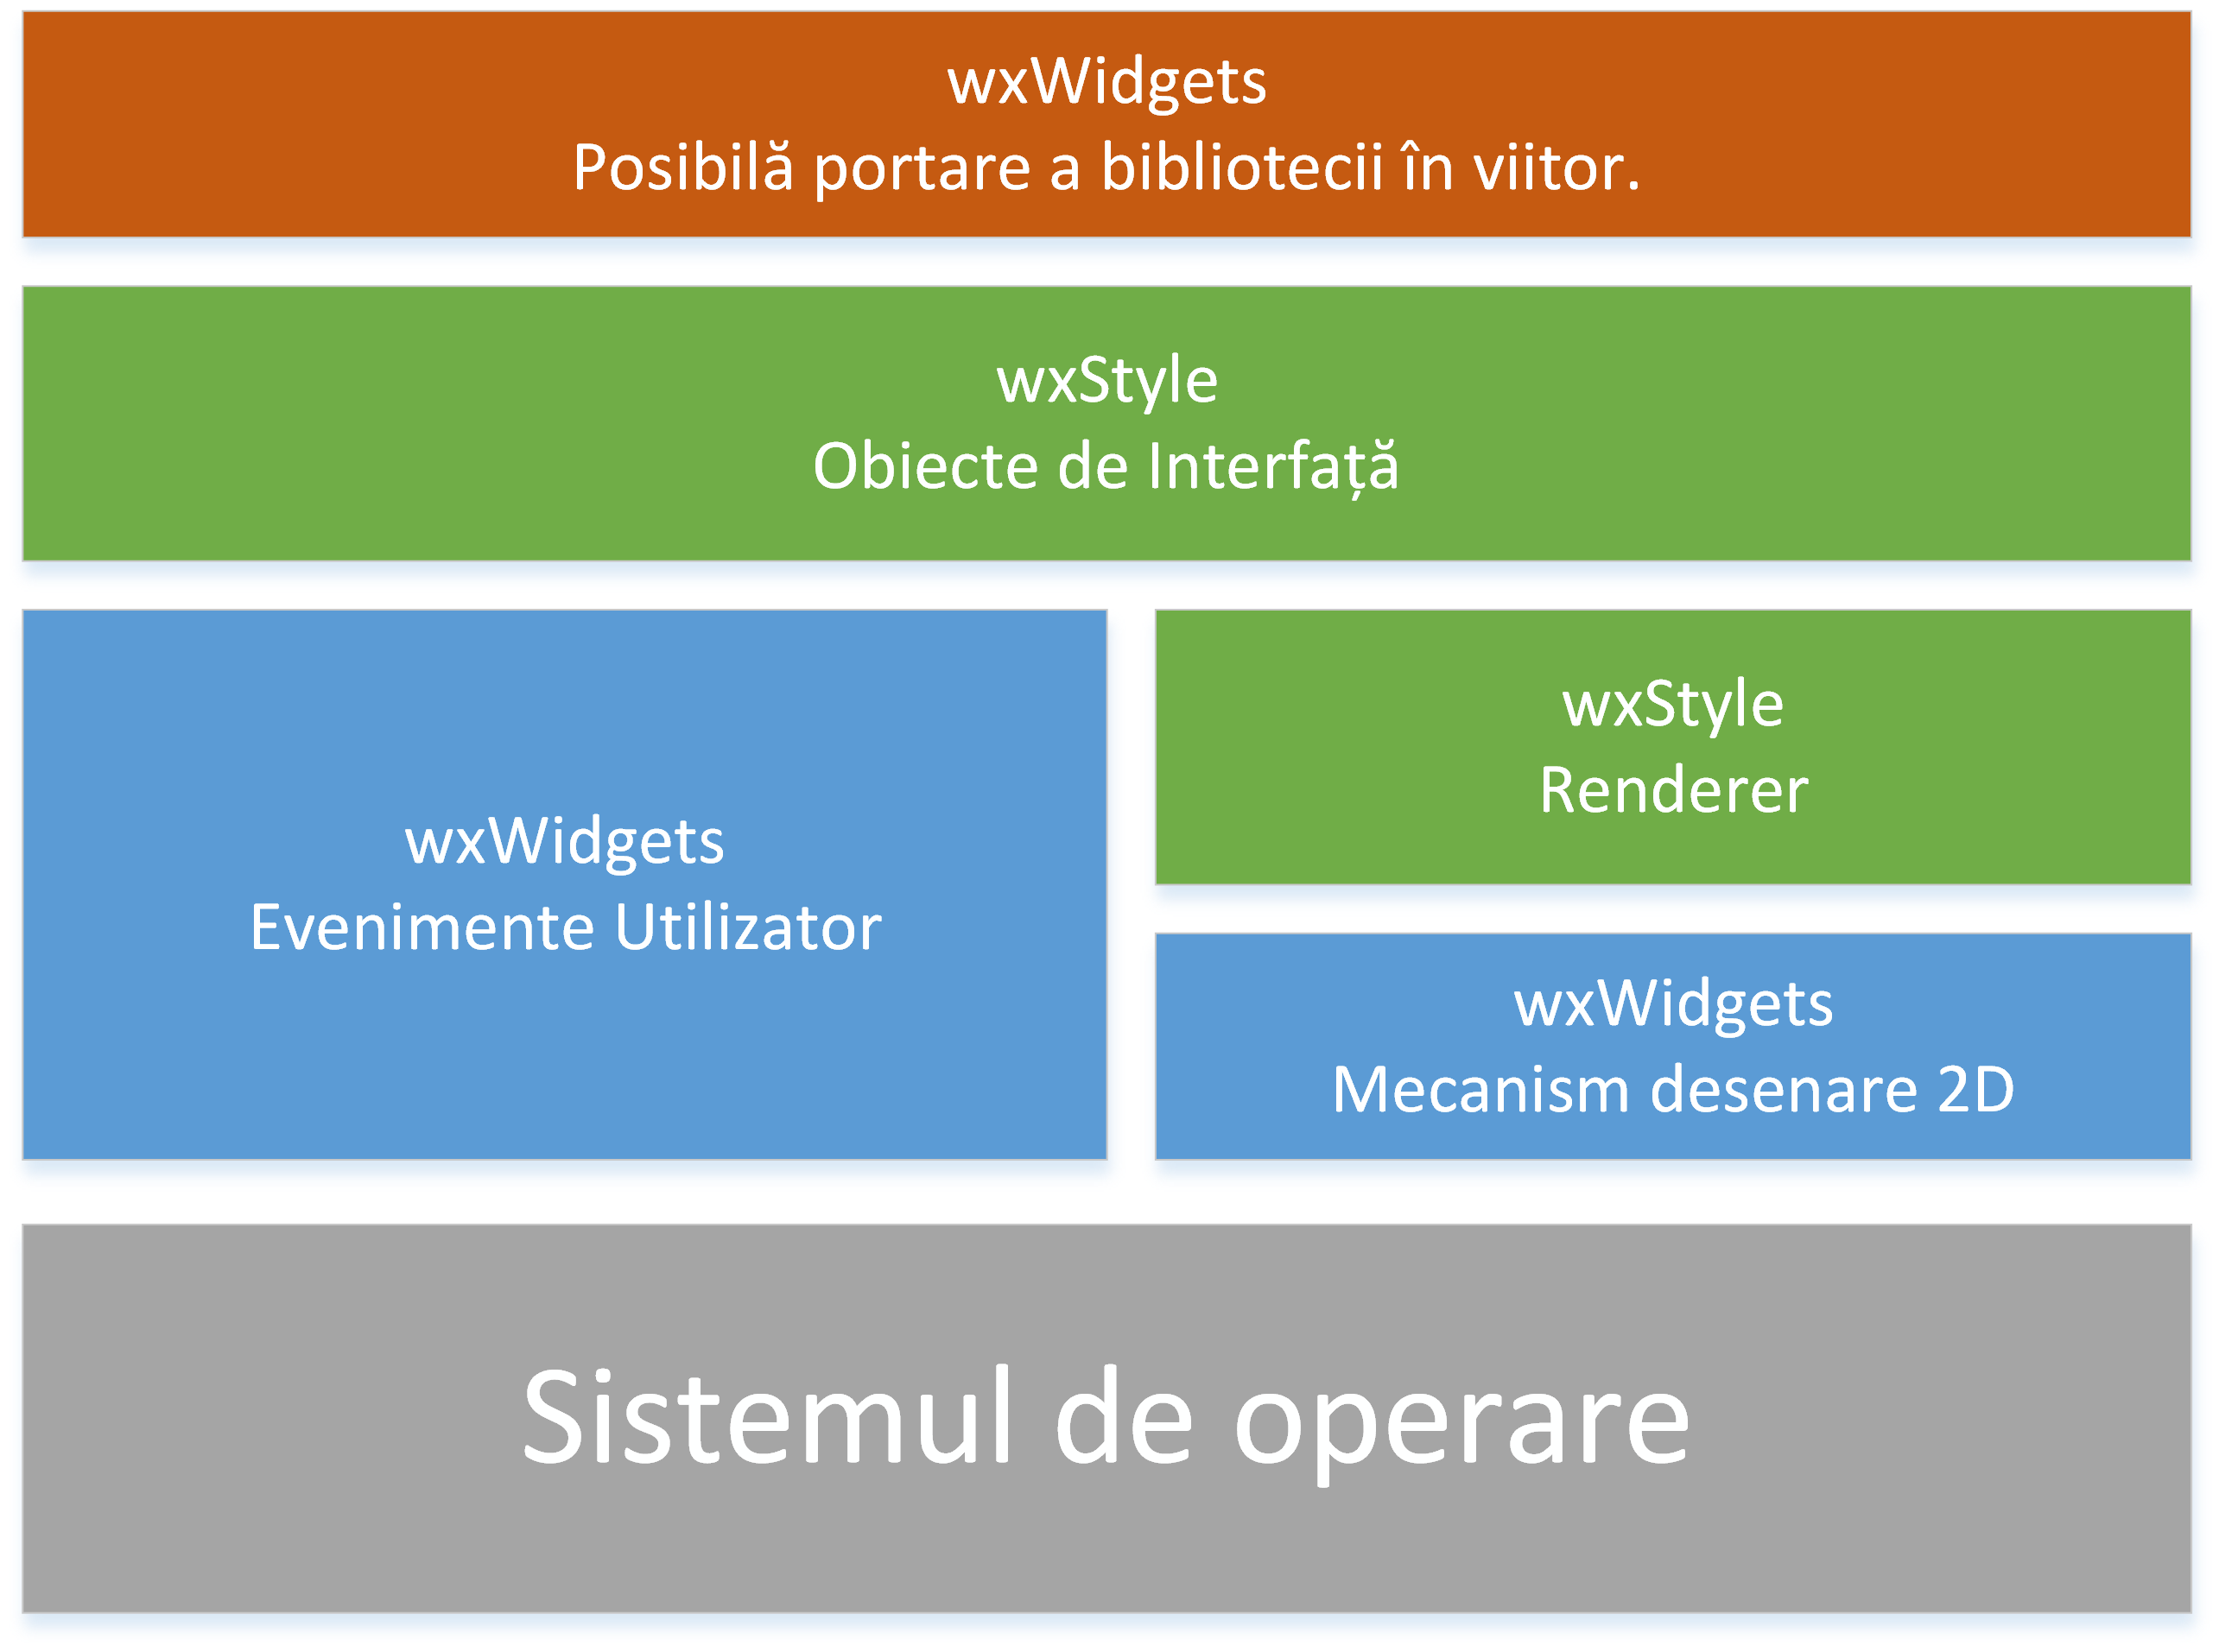
\includegraphics{img/ch2_arhitectura_bloc.png}
    \label{ch2_arhitectura_bloc}
    \caption{Arhitectura conceptual'a a bibliotecii wxStyle }
\end{figure}
\end{center}

\section{Mecanismului de stilizare}

Mecanismul de stilizare utilizeaz'a descrieri de stil pentru a specifica aspectele de prezentare ale unui obiect de interfa't'a. Un stil trebuie sa con'tin'a informatia necesar'a pentru:

\begin{enumerate}
\item Culorile de fundal si pentru text.
\item Font-ul utilizat la desenarea textului. 'In specifica'tia fontului includem: familia fontului, dimensiunea, greutatea fontului (sub'tire, normal sau bold) 'si 'inclina'tia fontului.
\item Umbra textului, care este descrisa printr-o deplasare relativ'a fa't'a de text 'si culoare.
\item Icoana utilizat'a op'tional de obiectul de interfa't'a va fi reprezentat'a prin numele imaginii.
\item Marginile interioare (numite si inset-uri), ce reprezint'a distan'ta dintre con'tinutul propriu-zis al unui obiect de interfa't'a 'si extremit'a'tile sale.
\item Aliniamentul textului at{\ia}t pe vertical'a c{\ia}t 'si pe orizontal'a.
\item Specificarea dac'a obiectul de interfa't'a este opac sau nu.
\item Un set de instruc'tiuni pentru desenarea fundalului.
\end{enumerate}

Urmatoarele reguli descriu modul de func'tionare al mecanismului de stilizare:

\begin{enumerate}
\item Toate obiectele de interfa't'a au ata'sate o procedur'a de desenare ce poate fi schimbat'a.
\item Toate obiectele de interfa't'a au ata'sat un stil complet, ce poate fi suprascris.
\item Defini'tiile de stil pot fi incomplete. Atunci c{\ia}nd unui obiect de interfa't'a i se ata'seaz'a un stil incomplet, con'tinutul acestuia va suprascrie doar acele tr'as'aturi care sunt definite.
\item Procedura de desenare ata'sat'a implicit unui obiect de interfa't'a utilizeaza stilul pentru a construi o reprezentare vizual'a.
\item Un fi'sier de stil con'tine mai multe stiluri ce pot fi ata'sate unei categorii de obiecte de interfa't'a (de exemplu tuturor butoanelor din aplica'tie).
\end{enumerate}

Setul de instruc'tiuni ata'sat unui stil descriu o primitiv'a de desenare 'impreuna cu parametrii acesteia. Este necesar'a posibilitatea desen'arii de imagini, forme 'si text cu dimensiuni 'si alinimente at{\ia}t relative c{\ia}t 'si absolute 'in cadrul unui obiect de interfa't'a.

\medskip

Componentele implementate 'in libr'aria wxStyle vor putea fi folosite 'impreun'a sau 'in locul celor implementate 'in cadrul libr'ariei wxWidgets. Un scop mai mare al acestei biblioteci, de'si imposibil de atins 'in cadrul lucr'arii de licent'a, este acela de a oferi o platform'a nou'a pentru wxWidgets, deasupra c'areia s'a poat'a fi portate toate obiectele de interfa't'a.
%
%% ==============================================================================
%%   Capitolul 3: Studiu Bibliografic
%% ==============================================================================
%
\chapter{Studiu Bibliografic}
\pagestyle{headings}

'In cadrul activit'a'tii de studiu bibliografic, am apelat la c'ar'ti de referin't'a 'in domeniul graficii pe calculator, a activit'a'tii de proiectare 'si dezvoltare a interfe'te'lor vizuale dar 'si a utiliz'arii eficiente a tehnologiilor alese pentru dezvoltarea proiectului.

\section{Grafica pe calculator}

\subsubsection{Computer Graphics: Principles and Practice Second Edition}

Probabil una dintre cele mai influente c'ar'ti introductive ale literaturii de specialitate, \emph{Computer Graphics: Principles and Practice Second Edition}\cite{computergraphics} a fost publicat'a pentru prima dat'a 'in anul 1995. Edi'tia a doua, introduce elemente de grafic'a 2D si 3D raster, grafic'a vectorial'a, interfe'te utilizator, anti-aliasing, algoritmi avansa'ti de desenare 'si o introducere 'in anima'tie.

\medskip

Trebuie s'a 'tinem cont de contextul 'in care cartea a fost scris'a, mai specific perioada anilor 95, c{\ia}nd calculatoarele personale asistau la o revolu'tie digital'a a tehnologiei 'si se putea vorbi pentru prima dat'a de no'tiuni precum interfe'te utilizator. Din acest motiv, capitolele \emph{Chapter 8: Input Devices, Interaction Techniques, and Interaction Tasks}, \emph{Chapter 9: Dialogue Design} 'si \emph{Chapter 10: User Interface Software} prezint'a fundamentele necesare proiect'arii 'si implement'arii unei arhitecturi pentru interfe'te utilizator. Autorii prezint'a conceptele de interac'tiune cu utilizatorul prin tehnici 'si task-uri de interac'tiune 'si modul de abstractizare al acestor activit'a'ti prin metafore.

\medskip

Capitolele \emph{Chapter 3: Basic Raster Graphics Algorithms for Drawing 2D Primitives} 'si \emph{Chapter 5: Geometrical Transformation} ofer'a informa'tia necesar'a implement'arii algoritmilor pentru desenare 'in dou'a dimensiuni. Pentru scopul acestui proiect, biblioteca wxWidgets 'impreun'a cu sistemul de operare ofer'a suportul necesar 'si suficient al primitivelor de desenare, iar aceste capitole sunt doar pentru a dezvolta o mai bun'a 'in'telegere a detaliilor.

\section{Proiectarea 'si dezvoltarea de interfe'te utilizator vizuale}

Despre proiectarea 'si dezvoltarea interfe'telor utilizat'or vizuale au fost scrise numeroase c'ar'ti, articole, studii, etc. Pentru proiectul de fa't'a, cele mai am ales trei dintre cele mai cunoscute

\subsubsection{The Old New Thing: Practical Development Throughout the Evolution of Windows}

\emph{The Old New Thing: Practical Development Throughout the Evolution of Windows}\cite{theoldnewthing} a fost scris'a 'in anul 2007 de c'atre Raymond Chen, unul dintre cei mai vechi dezvoltatori Microsoft. Autorul  'inc'a de la apari'tia primelor versiuni de Windows. Cartea sa este 'imp'ar'tit'a in scurte recolec'tii 'si povestiri care ofer'a un context deciziilor luate de echipa Microsoft la proiectarea interfe'telor vizuale pentru sistemele de operare Windows.

\medskip

Raymond Chen poveste'ste dificult'a'tile utilizatorilor sistemului de operare, frustr'arile 'si reac'tiile acestora 'in momentul confrunt'arii cu interfa'ta neintuitiv'a 'si necizelat'a a primelor versiuni de Windows. Autorul explic'a 'si deciziile luate de echipa responsabil'a pentru dezvoltarea interfe'tei grafice a sistemului de operare pentru rezolva problemele utilizatorilor. Cartea este relevant'a proiectului deoarece prezint'a modurile 'in care utilizatorii interactioneaz'a cu un sistem software, care sunt obieceiurile 'si instinctele lor 'si ce solu'tii se pot adopta pentru a asigura o interac'tiune c{\ia}t mai u'soar'a cu sistemul. Aceste solu'tii necesit'a un set de unelte pentru a fi implementate, printre care se num'ar'a si biblioteca wxStyle.

\subsubsection{Designing Interactive Systems: a comprehensive guide to HCI and interaction design}

Una dintre cele mai renumite c'ar'ti din domeniuni interac'tiunii om - calculator, cartea este 'imp'ar'tit'a 'in studii de caz extrase din experien'ta autorului. Fiecare studiu prezint'a o provocare 'in ceea ce prive'ste arhitectura 'si implementarea unui sistem interactiv. Printre capitole care parcurg tehnicile esentiale in dezvoltarea aplica'tiilor interactive, autorul atinge 'si subiecte precum design-ul paginilor web 'si experien'ta utilizatorului. Prin experien't'a utilizator 'in'telegem emo'tiile 'si atitudinea utilizatorului fa't'a de sistem. La fel ca 'in cazul c'ar'tii lui Raymond Chen, aceast'a carte ajut'a la modelarea bibliotecii wxStyle prin definirea scopului si problemelor pe care biblioteca trebuie s'a le rezolve.

\subsubsection{Designing the user interface: strategies for effective human-computer interaction}

Aceast'a carte ofer'a o introducere aprofundat'a 'in domeniul interac'tiunii om - calculator. O echip'a de autori 'i'si aduc experien'ta prezent{\ia}nd cele mai bune practici 'si principii moderne 'in dezvoltarea aplica'tiilor dinamice. Cartea atac'a probleme contemporane precum experien'ta utilizatorului, re'tele de socializare, con'tinut generat de utilizatori, precum 'si probleme de securitate 'si spam. Cartea este dedicat'a 'in special platformelor mobile 'si web, dar principiile 'si practicile prezentate se aplic'a 'in egal'a m'asura aplica'tiilor desktop. Biblioteca wxStyle are rolul de a face posibile aceste practici 'in contextul de dezvoltare wxWidgets.

\subsubsection{Alte biblioteci 'si arhitecturi similare}

'In plus fa't'a de aceste c'ar'ti, am studiat bibliotecile \emph{Qt}, \emph{CEGUI (Crazy Eddie`s GUI System)}, libr'aria \emph{Swing} a limbajului Java 'si limbajele HTML 'si CSS. Toate aceste libr'arii sau limbaje au 'in comun nu doar suportul flexibil pentru construirea de obiecte de interfa't'a stilizabile, dar si separarea clar'a 'intre descrierea stilului utilizat la prezentarea unui obiect si implementarea acestuia. Aceste arhitecturi ofer'a o referin't'a 'si o funda'tie solid'a pentru deciziile luate 'in acest proiect.

\section{Tehnologii}

Aceast'a sec'tie cuprinde bibliografia referitoare at{\ia}t la tehnologiile utilizate de biblioteca wxStyle, c{\ia}t 'si exemple de tehnologii ce pot fi implementate folosind aceasta bibliotec'a.

\subsubsection{Cross-Platform GUI Programming with wxWidgets}

Biblioteca wxStyle este implementa'ta deasupra bibliotecii wxWidgets, deci este necesar'a o 'in'telegere profund'a a arhitecturii 'si implement'arii acesteia din urm'a.

\medskip

Singura carte ce trateaz'a biblioteca wxWidgets este cea scris'a de autorul original al bibliotecii Julian Smart, 'si este intitulat'a \emph{Cross-Platform GUI Programming with wxWidgets}\cite{wxwidgetsguide}. Aceast'a carte 'incepe prin a prezenta scopul original al bibliotecii: acela de a oferii dezvoltatorilor de aplica'tii portabile pentru ma'sini desktop sau mobile un set de unelte necesare dezvolt'arii de aplica'tii vizuale. Capitolele ce urmeaz'a prezint'a toate aspectele bibliotecii, 'incep{\ia}nd cu funda'tiile dezvolt'arii de aplica'tii vizuale prin procesarea de evenimente si utilizarea de obiecte de interfa't'a, apoi continu{\ia}nd cu capitole ce trateaza interna'tionalizarea, scrierea de programe paralele 'si utilizarea socket-urilor pentru a scrie programe ce interac'tioneaz'a cu re'teaua.

\medskip

Capitolele relevante acestei lucr'ari sunt \emph{Chapter 3 Event Handling}, \emph{Chapter 4 Window Basics}, \emph{Chapter 5 Drawing and Printing} 'si \emph{Chapter 6 Handling Input}. Capitolul 3 prezint'a sistemul de procesare a evenimentelor implementat 'in biblioteca wxWidgets. Acesta cuprinde utilizarea mecanismului de capturare 'si procesare de evenimente at{\ia}t dinamic c{\ia}t 'si static, generarea de evenimente 'si construirea unor tipuri noi de evenimente. Capitolul 4 ofera o privire de ansamblu asupra anatomiei unei ferestre. Informa'tiile din acest capitol sunt folositoare pentru implementarea propriei ferestre stilizabile. Capitolul 5 cuprinde aproape toate detaliile necesare implement'arii procesului de prezentare prin descrierea uneltelor de desenare 2D 'si a modului de utilizare al acestora. Capitolul 6 prezint'a modul de tratare al evenimentelor generate de interac'tiunea utilizatorului cu aplica'tia. Aceste evenimente de nivel jos (dispozitiv mouse 'si tastatur'a) pot fi folosite pentru a implementa logica fiec'arui obiect de interfa't'a.

Aceast'a carte este completat'a de wiki-ul\footnote{http://wiki.wxwidgets.org/} bibliotecii wxWidgets, 'impreun'a cu documenta'tia oficial'a\footnote{http://docs.wxwidgets.org/3.0/} a API-ului 'si forumul\footnote{http://forums.wxwidgets.org/} comunit'a'tii.

\subsubsection{The C++ Programming Language}

Cartea de referin'ta a limbajului C++ se numeste \emph{The C++ Programming Language}, iar edi'tia a patra a fost publicat'a de c'atre autorul limbajului Bjarne Stroustrup 'in anul 2013. Aceast'a edi'tie este relevan'ta pentru standardul C++11 al limbajului 'si con'tine informa'tii despre toate aspectele limbajului de programare de la tipuri de date primitive, operatori, expresii 'si instruc'tiuni p{\ia}n'a la mecanisme avansate de abstractizare precum clase 'si continutul bibliotecii standard.

\medskip

Aceast'a carte este esen'tial'a pentru a 'in'telege limbajul C++ 'in 'intregime 'si serve'ste rolul de referin't'a pentru orice aspect al limbajului. Cartea poate fi considerat'a o versiune mai u'sor de citit 'si 'in'teles, dar mai restr{\ia}ns'a din punct de vedere al con'tinutului, a standardului C++.

\subsubsection{Exceptional C++}

Una din cele mai renumite c'ar'ti ce trateaz'a subiectul utiliz'arii corecte a limbajului C++ este \emph{Exceptional C++}\cite{exceptional_cpp} scris'a de Herb Sutter. Autorul face parte din comisia de standardizare a limbajului 'si este o figur'a renumit'a pentru prezent'arile sale 'in cadrul conferin'telor de specialitate, pentru c'ar'tile considerate de c'ap'at{\ia}i pentru orice programator C++ 'si pentru articolele sale celebre despre limbajul C++ intitulate colectiv \emph{Guru of the Week}.

\medskip

Cartea este structurat'a ca o serie de 'intreb'ari 'si r'aspunsuri pe tema utiliz'arii corecte a limbajului, 'in special securitate, tratarea excep'tiilor 'si dezvoltarea de arhitecturi stabile 'si eficiente prin utilizarea corect'a a tr'as'aturilor limbajului 'si a libr'ariei standard.

\subsubsection{Effective C++, More Effective C++ 'si Effective STL}

Aceste trei c'ar'ti\cite{effective_cpp}\cite{more_effective_cpp}\cite{effective_stl} scrise de autorul Scott Meyers fac parte din biblioteca obligatorie a programatorului C++, 'impreun'a cu c'ar'tile lui Herb Sutter. Aceste c'ar'ti trateaz'a utilizarea corect'a a limbajului 'si a tr'as'aturilor sale mai mult sau mai pu'tin obscure. C'ar'tile sunt organizate in item-uri, fiecare prezent{\ia}nd o regul'a general valabil'a care poate fi aplicat'a 'in orice situa'tie pentru a garanta corectitudinea unui program.

\medskip

Primele dou'a c'ar'ti se preocup'a de utilizarea corect'a a nucleului limbajului 'si metodelor sale de abstractizare, de utilizarea corect'a a claselor, de suprascrierea corect'a a operatorilor 'si de evitarea gre'selilor uzuale. Scott Meyers acoper'a 'si problema administr'arii memoriei prin prezentarea metodei RAII 'si a pointer-ilor inteligen'ti din biblioteca standard. Cartea din urm'a trateaz'a utilizarea corect'a a libr'ariei standard printre care cunoasterea diverselor tipuri de iteratori 'si familiarizarea cu colec'tiile 'si preforman'tele acestora.

\subsubsection{Large-Scale C++ Software Design}

Cartea \emph{Large-Scale C++ Software Design}\cite{largescalecpp}, scris'a de autorul John Lakos 'in anul 1997 adreseaz'a problemele des 'int{\ia}lnite 'in dezvoltarea aplica'tiilor de dimensiuni extinse folosind limbajul C++. Deoarece biblioteca wxStyle con'tine un num'ar relativ ridicat de fi'siere surs'a (aproximativ 70 la momentul scrierii acestei documenta'tii) care implementeaz'a componente distincte (obiecte de interfa't'a, instruc'tiuni de desenare, obiecte de prezentare, analizator de fi'siere de stil) ce formeaz'a diverse rela'tii de dependin't'a (cum ar fi rela'tiile de mo'stenire 'si agregare) putem considera proiectul suficient de extins pentru a beneficia de informa'tiile prezente 'in aceast'a carte.

\medskip

Printre regulile fundamentale recomandante de John Lakos se num'ar'a evitarea expunerii implement'arilor prin metoda pointerilor opaci sau pointerilor c'atre implementare (PIMPL idiom), minimizarea dependin'telor 'intre module folosind declara'tii 'inainte (forward declarations), evitarea categoric'a a dependin'telor ciclice 'si testarea independent'a a modulelor. Alte informa'tii detaliate despre structura limbajului ajut'a la dezvoltarea de aplica'tii sigure (prin evitarea greselilor subtile), usor de 'intre'tinut 'si de extins (prin structurarea aplica'tiilor 'in arhitecturi flexibile).

\subsubsection{User interface contrast filter}

Prin adaugarea suportului pentru stilizare, biblioteca wxStyle ofer'a dezvoltatorilor posibilitatea de a schimba dinamic, 'in timpul rul'arii unei aplica'tii inf'a'ti'sarea obiectelor de interfa't'a. Aceast'a nou'a posibilitate deschide por'tile unei genera'tii noi de aplica'tii care se pot adapta la factori externi precum luminozitatea sau temperatura mediului.

\medskip

O astfel de tehnologie este patentat'a de Apple\cite{uicontrast} 'si specific'a o metod'a prin care aplica'tiile vizuale ce ruleaz'a pe dispozitive mobile 'i'si pot schimba contrastul pentru a se adapta la condi'tii de vizibilitate redus'a determinate de luminozitatea extern'a. De'si aceast'a tehnologie este ap'arat'a de legile privind dreptul de autor 'si este curent de'tinut'a de Apple, ea este un exemplu deosebit de relevant pentru scopul existen'tei bibliotecii wxStyle. Mai precis, aplica'tiile moderne au nevoie de mecanisme u'sor de utilizat pentru manipularea dinamic'a a interfe'telor vizuale.
%
%% ==============================================================================
%%   Capitolul 4: Analiza si Fundamentare Teoretica
%% ==============================================================================
%
\chapter{Analiz'a Teoretic'a}
%\pagestyle{headings}
%
\section{Introducere}
%
%\begin{center}
%\begin{figure}[h]
%    \centering
%    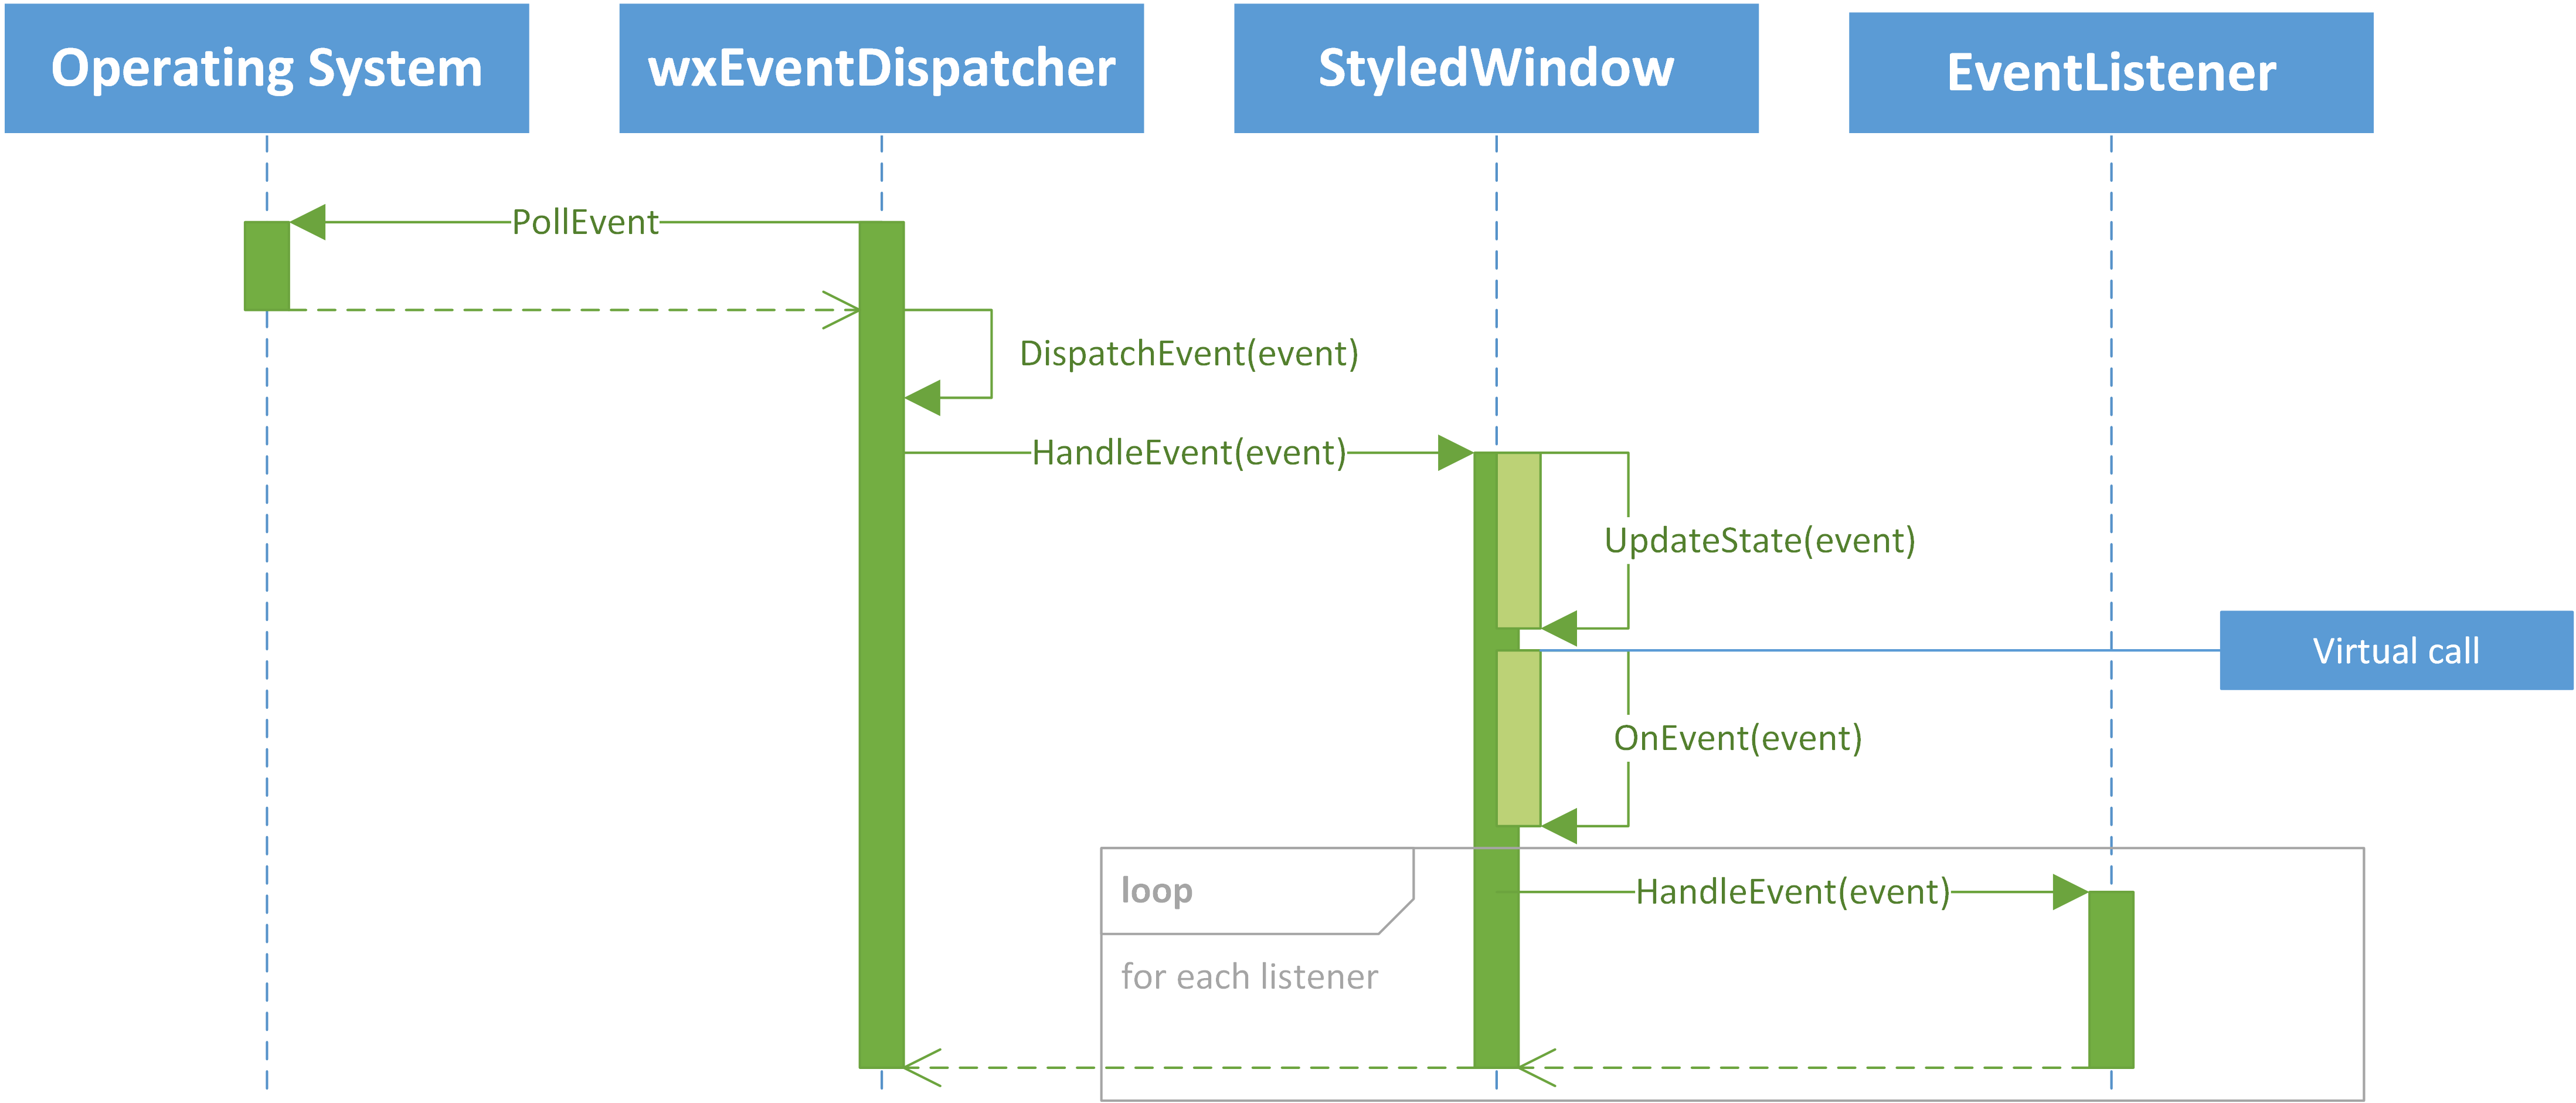
\includegraphics[scale=0.9]{img/ch4_seq_event_processing.png}
%    \label{fig0401}
%    \caption{UML Class Diagram pentru Renderer}
%\end{figure}
%\end{center}
%

Pentru a asigura o bun'a desf'a'surare a activit'a'tii de dezvoltare 'si 'intre'tinere a oric'arui proiect, pentru a asigura flexibilitate la schimb'ari 'in domeniul cerin'telor 'si pentru a preveni hazarduri ulterioare, este necesar'a o analiz'a profund'a 'si am'anun'tit'a a proiectului 'si a componentelor sale 'inainte de 'inceperea implement'arii.

\medskip

Acest capitol 

\begin{itemize}
\item {\bf Cerin'tele proiectului} sunt structurate 'in cazuri de utilizare. 'Incep{\ia}nd cu analiza cerin'telor ne asigur'am ca proiectul atinge ni'ste scopuri bine definite f'ar'a a irosi timp 'in implementarea unor tr'as'aturi nenecesare. 'In plus, putem pleca de la cerin'tele ini'tiale pentru a scrie teste 'si a valida finalizarea proiectului.
\item {\bf Analiza arhitecturilor similare} presupune suprapunerea tehnologiilor deja existente peste cerin'tele proiectului 'si a decide dac'a deciziile luate 'in dezvoltarea altor arhitecturi se aplic'a la acest proiect. 'In cazul 'in care mai multe arhitecturi diferite se prezint'a favorabile, vom decide care este mai potrivit'a.
\item {\bf Prezentarea arhitecturii finale}
\item {\bf Descrierea componentelor}
\end{itemize}

\clearpage

\section{Cazuri de utilizare}

Pentru a modela cerin'tele proiectului, prezent'am urm'atoarele cazuri de utilizare ce au rolul de a documenta cerin'tele func'tionale ale bibliotecii wxStyle.

\begin{figure}[H]
	\centering 
	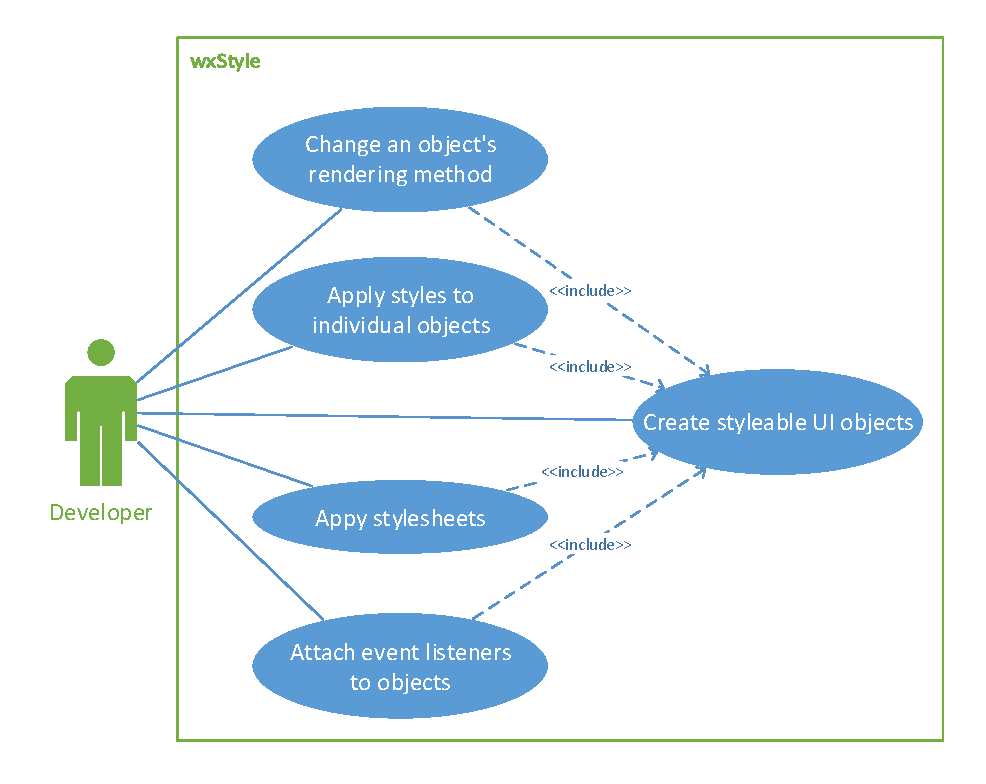
\includegraphics{img/use_case.pdf}
	\label{fig0402}
    \caption{Diagrama UML a cazurilor de utilizare}
\end{figure}

%Cazurile de utilizare prezentate 'in figura \ref{fig0402} acoper'a 

%\clearpage

\subsection{Crearea unui obiect de interfa't'a}
\textbf{Precondi'tie:} Utilizatorul a configurat un mediu de dezvoltare care are acces la bibliotecile wxWidgets 'si wxStyle.
\begin{enumerate}
\item Utilizatorul preg'ate'ste o aplica'tie vizual'a wxWidgets prin implementarea 'si instan'tierea unui wxApp.
\item Utilizatorul declar'a o variabil'a cu unul din tipurile de date ale obiectelor stilizabile 'si 'ii asigneaz'a o instan'ta a acestui tip utiliz{\ia}nd constructorul.
\item Utilizatorul amplaseaz'a obiectul de interfa't'a 'in cadrul unei ferestre, utiliz{\ia}nd constr{\ia}ngeri de amplasare, printr-un proces identic cu amplasarea obiectelor de interfa't'a implementate in biblioteca wxWidgets.
\item Utilizatorul compileaz'a 'si ruleaz'a aplica'tia.
\end{enumerate}
\textbf{Rezultat:} Obiectul de interfa't'a este prezent in cadrul ferestrei.

\subsection{Stilizarea unui obiect de interfa't'a}
\textbf{Precondi'tie:} Parcurgerea cazului de utilizare intitulat \emph{Crearea unui obiect de interfa't'a}.

\begin{enumerate}
\item Utilizatorul construie'ste o instan't'a a clasei \emph{Style} 'si apeleaz'a metodele asociate cu setarea defini'tiilor de stilizare.
\item Utilizatorul ata'seaz'a stilul la un obiect de interfa't'a stilizabil.
\item Utilizatorul compileaz'a 'si ruleaz'a aplica'tia.
\end{enumerate}
\textbf{Rezultat:} Obiectul de interfa't'a este desenat conform defini'tiilor de stil specificate 'in structura de stil.

\subsection{Modificarea procesului de prezentare al unui obiect de interfa't'a}
\textbf{Precondi'tie:} Parcurgerea cazului de utilizare intitulat \emph{Crearea unui obiect de interfa't'a}.
\begin{enumerate}
\item Utilizatorul declar'a o nou'a clasa ce implementeaz'a interfa't'a numit'a \emph{Renderer}.
\item Utilizatorul implementeaz'a metoda \emph{Draw} a acestei clase folosind primitivele de desenare oferite de wxWidgets 'si instruc'tiunile de desenare oferite de wxStyle pentru a desena o reprezentare grafic'a a obiectului de interfa't'a conform st'arii acestuia.
\item Utilizatorul ata'seaz'a o instan't'a a acestei clase unui obiect de interfa't'a stilizabil.
\item Utilizatorul compileaz'a 'si ruleaz'a aplica'tia.
\end{enumerate}
\textbf{Rezultat:} Sistemul prezin'ta obiectul de interfa't'a 'in func'tie de starea sa 'si metoda de desenare implementat'a 'in cadrul clasei de prezentare.

\subsection{Schimbarea aspectului aplica'tiei}
\textbf{Precondi'tie:} Parcurgerea cazului de utilizare intitulat \emph{Crearea unui obiect de interfa't'a}.
\begin{enumerate}
\item Utilizatorul creaz'a op'tional mai multe obiecte de interfa't'a pe care le amplaseaz'a 'in cadrul unei ferestre.
\item Utilizatorul creaz'a o structur'a \emph{Stylesheet}.
\begin{enumerate}
  \item Utilizatorul construie'ste mai multe structuri de tipul \emph{Style} cu scopul de a le asocia unui tip de obiecte de interfa't'a.
  \item Utilizatorul ata'seaz'a stilurile structurii \emph{Stylesheet} 'si le asociaz'a c{\ia}te un nume unic.
  \item Utilizatorul face asocierea dintre tipul obiectului de interfa't'a 'si stilul dorit, ambele identificate prin numele lor, utiliz{\ia}nd metodele de asociere ale structuri \emph{Stylesheet}
\end{enumerate}
\item Utilizatorul aplic'a structura \emph{Stylesheet} prin inregistrarea sa la nivel global.
\end{enumerate}
\textbf{Rezultat:} 'In urma rul'arii aplica'tiei, toate obiectele de interfa't'a stilizabile ce nu au asociate stiluri sau clase de prezentare specificate de utilizator vor fi prezentate conform stilurilor asociate tipului lor din structura \emph{Stylesheet} 'inregistrat'a la nivel global.

\subsection{Procesarea evenimentelor}
\textbf{Precondi'tie:} Parcurgerea cazului de utilizare intitulat \emph{Crearea unui obiect de interfa't'a}.
\begin{enumerate}
\item Utilizatorul identific'a sursa evenimentului, care poate fi eveniment de interac'tiune utilizator sau eveniment generat de un obiect de interfa't'a.
\item Utilizatorul declar'a o nou'a clas'a care extinde interfa't'a de tip \emph{Listener} asociat'a evenimentului.
\item Utilizatorul implementeaz'a acea metod'a care proceseaz'a evenimentul dorit.
\item Utilizatorul ata'seaz'a o instan't'a a acestei clase unuia sau mai multora obiecte de interfa't'a.
\end{enumerate}
\textbf{Rezultat:} Metoda implementa't'a de utilizator este apelat'a 'in momentul producerii unui eveniment de tipul corect.

% Motivul utilizarii
\subsection{Procesare evenimentelor}
Motivul pentru implementarea unui alt mecanism de procesare al evenimentelor este de a oferi posibilitatea mai multor obiecte sa raspunda la evenimente. In momentul in care o rutina de procesare al evenimentului este legat'a de un anumit tip de eveniment si un anumit obiect, evenimentele de acel tip produse de acel obiect nu vor mai putea fi procesate de alta rutin'a. Acest lucru ingreuneaz'a biblioteca wxStyle, deoarece obiecte precum ResizeHandler 'si DragHandler trebuie sa poata intercepta evenimentele produse de dispozitiv-ul mouse f'ar'a a intrerupe propagarea acestora c'atre obiectul c'arora le este destinat. Dac'a aceste evenimente nu ar ajunge la obiectul destinatar, acesta nu ar putea s'a-'si actualizeze starea sau s'a genereze evenimente abstracte specifice obiectului precum ap'asarea unui buton sau mutarea indicatorului de text 'in interiorul unui obiect de interfa't'a pentru introducerea de text.

Cel mai popular mecanism de distribuire a unui eveniment este cel bazat pe sablonul Observer. Acest mecanism presupune prezen'ta a dou'a componente: un produc'ator de evenimente 'si mai mul'ti 'ascult'atori de evenimente. Ascult'atorii se pot 'inregistra la produc'ator pentru a fi notifica'ti 'in cazul 'in care un nou eveniment este produs. La orice moment, un ascult'ator se poate deinregistra de la produc'ator. Produc'ator men'tine o list'a de ascult'atori. Ac'tiunile de inregistrare si deinregistrare se traduc 'in ac'tiuni de manipulare a listei precum ad'augarea unui noi observator sau 'stergerea unuia deja existent. Notificarea observatorilor presupune apelarea unei metode a obiectului observator. Aceste metode sunt predefinite de interfa't'a observatorului. Fiecare produc'ator accept'a doar un anumit tip de observator, pentru a asigura prezen'ta metodelor de procesare. 'In momentul gener'arii unui nou eveniment, produc'atorul notific'a toti observatorii. Utiliz{\ia}nd acest mecanism, putem procesa acela'si eveniment din locuri multiple.

O problem'a la mecanismul de observator pentru procesarea evenimentelor este ordinea 'in care observatorii sunt notifica'ti de prezent'a unui eveniment. Dorim s'a ne asigur'am c'a obiectele de interfa't'a c'arora le este destinat evenimentul au ocazia s'a 'il proceseze 'inaintea altor observatori inregistrati de c'atre utilizatori. Din acest motiv, evenimentele sunt procesate 'in trei etape:

1. Clasa StyledWindow primeste evenimentul de la biblioteca wxStyle prin mecanismul standard wxWidgets. In cadrul acestei rutine, StyledWindow adjusteaz'a starea obiectului precum: dac'a este sau nu ap'asat, daca dispozitivul mouse se afl'a sau nu deasupra obiectului, etc.
2. StyledWindow apeleaza metoda virtuala On{Event} care este implementat'a (la nevoie) de tipul real al obiectului. In acest fel, obiectele de interfa't'a au ocazia s'a interpreteze evenimentele pentru a-'si 'intre'tine propria stare intern'a.
3. StyledWindow notific'a to'ti observatorii inregistra'ti pentru evenimentul respectiv. Ordinea 'in care ace'stia sunt notifica'ti este aceea 'in care ei s-au 'inregistrat.

Deoarece clasa StyledWindow are responsabilitatea de a 'intre'tine starea obiectului, de a apela metoda virtual'a de procesare 'si de a notifica to'ti observatorii asigur'a corectitudinea proces'arii evenimentelor. Obiectele specifice de interfa't'a nu au responsabilitatea de a 'intre'tine o list'a de observatori sau de a procesa evenimentele 'intr-o anumit'a ordine.

% Rough Ideas
\subsection{Stilul implicit}
Pentru a putea utiliza u'sor 'si sigur mecanismul de stilizare, avem nevoie de garan'tia c'a defini'tiile obligatorii ale unui stil exist'a. Defini'tiile obligatorii sunt acele defini'tii f'ar'a de care nu se poate construi o reprezentare a obiectului de interfa't'a. De exemplu: defini'tiile pentru font, culoarea planului prioritar (foreground), combina'tia de defini'tii care descriu opacitatea 'si modul de prezentare al fundalului. Aceste defini'tii, dac'a nu sunt explicit setate, trebuie s'a aibe o valoare predefinit'a. Aceast'a valoare predefinit'a provine de la stilul implicit al bibliotecii wxStyle. Prin mecanismul de mo'stenire al stilurilor, toate defini'tiile setate manual de utilizator se vor aplica deasupra stilului implicit. Stilul implicit este urm'atorul:

% BLA, BLA, BLA

De asemenea, mecanismul de stilizare prin fi'siere de stil \emph{stylesheets} trebuie sa poata stiliza 'intreaga aplica'tie la orice moment 'in timpul rul'arii acesteia. Acest lucru presupune modificarea tuturor obiectelor de interfata ce nu au stiluri sau proceduri de prezentare predefinite din componen'ta aplica'tiei. Implementarea acestui mecanism poate fi facut'a 'in dou'a moduri:

1. Prin men'tinerea unei liste de obiecte vizuale care s'a con'tin'a toat'e obiectele de interfa't'a din componen'ta aplica'tiei. La momentul stiliz'arii aplica'tiei, toate obiectele din list'a vor fi parcurse, iar stilurile sau metodele lor de prezentare vor fi actualizate.
2. Prin men'tinerea unei liste de stiluri implicite, indexate dup'a tipul obiectului de interfa't'a c'aruia 'ii sunt asociate. Schimbarea stilului aplica'tiei implic'a updatarea stilulurilor din aceast'a lista. La momentul prezent'arii unui obiect ce nu are un stil sau un obiect de prezentare definit de utilizator, acesta interogheaz'a lista de stiluri 'si obiecte de prezentare standard.

Metoda num'arul 1 implic'a stocarea 'in memorie a tuturor instan'telor de obiecte vizuale din aplica'tie, 'intr-o structur'a de date de tip list'a. Aceast'a list'a este greu de 'intre'tinut deoarece obiectele trebuiesc 'sterse din list'a 'in momentul 'in care acestea sunt distruse. Mai mult, modificarea unui stil predefinit implic'a parcurgerea 'intregii liste, indiferent dac'a obiectul este vizibil sau nu. Totu'si, lista va fi parcurs'a o singur'a dat'a pentru fiecare schimbare 'in setul de stiluri predefinite ale aplica'tiei. De cele mai multe ori, acest lucru se va realiza de doua ori: prima data pentru setarea stilului implicit al bibliotecii, iar a doua oara pentru setarea stilurilor specificate implicit de c'atre utilizator. Pentru a nu suprapune stilul implicit peste un stil setat de utilizator, toate obiecte de interfa't'a vor trebui augmentate cu un membru boolean care s'a indice dac'a stilul sau obiectul de prezentare al obiectului de interfa't'a este sau nu setat explicit de c'atre utilizator.

Metoda num'arul 2 are avantajul c'a nu necesit'a men'tinerea unei structuri de date suplimentare pentru stocarea instan'telor obiectelor de interfa't'a. 'In schimb, aceast'a metoda presupune stocarea stilurilor, 'si delegarea opera'tiei de citire a stilurilor c'atre fiecare obiect de interfa't'a. In mod similar primei metode, aceast'a metod'a necesit'a augmentarea cu membrul suplimentar care s'a disting'a dintre stiluri si obiecte de prezentare setate de utilizator, si cele implicite. Doar obiectele ce nu au stiluri setate explicit vor apela la cele implicite. Accesul la stilurile si obiectele de interfa't'a implicite se poate face printr-o instan'ta global'a 'si unic'a a unei clase ce are singurul rol de a stoca aceast'a informa'tie. O alt'a metod'a este de a oferi tuturor obiectelor de interfa't'a o instan'ta a unei clase ce poate "produce" stiluri si obiecte de prezentare specializate pentru tipul obiectului de interfa't'a. Folosim verbul "produce", deoarece dorim ca instantele de stiluri sa poat'a varia 'in timpul rul'arii, deci nu putem trimite instan'te concrete. Mai degrab'a trimitem un obiect care poate construi instan'te variabile 'in timpul rul'arii.




%\section{Design patterns}
%
%\subsection{Observer}
%
%\subsection{Singleton}
%
%\subsection{Factory}

%
%% ==============================================================================
%%   Capitolul 5: Proiectare de Detaliu si Implementare
%% ==============================================================================
%
\chapter{Implementare}
\pagestyle{headings}

\section{Considera'tii generale}
Coding conventions, file and folder arangements, build system.

\subsection{Pointer to Implementation (PIMPL)}
Compilation time reducer, proper encapsulation, etc.

\subsection{Managementul resurselor (RAII)}

\section{Infrastructur'a}

% ==============================================================================
%   Obiecte de interfata
% ==============================================================================

\section{Obiecte de Interfa't'a}

Datorit'a implement'arii bibliotecii wxWidgets, mai precis decizia de a folosi obiecte de interfa't'a native 'in spatele unor interfe'te abstractizate, modul de prezentare al acestor obiecte este nativ platformei pe care se executa aplica'tia. De'si o tr'as'atur'a avantajoas'a a bibliotecii, acest lucru 'impedic'a specializarea prezent'arii obiectelor. Singura solu'tie este reimplementarea obiectelor de interfa't'a cu suport pentru stilizare incorporat. Obiectele implementate de biblioteca wxStyle sunt prezentate in tabelul \ref{comp_tech_int}

\begin{center}
\begin{figure}[H]
    \centering
    \begin{tabular}{ |p{2.5cm}|p{3cm}|p{9.1cm}| }
        \hline
        \textbf{wxWidgets} & \textbf{wxStyle} & \textbf{Descriere} \\
        \hline
        wxWindow            & StyledWindow      & R'ad'acina ierarhiei  \\
        wxFrame             & StyledFrame       & Reprezint'a o fereastr'a (window)\\
        wxStaticText        & StyledLabel       & Reprezint'a informa'tie sub forma de text 'si icoan'a \\
        wxButton            & StyledButton      & Permite ac'tionarea unui buton prin ap'asare \\
        wxCheckBox          & StyledCheckBox    & Permite reprezentarea unei valori logice \\
        wxTextCtrl          & StyledTextBox     & Permite editarea de text \\
        \hline
    \end{tabular}
    \caption{Asociere 'intre obiectele de interfa't'a implementate in wxStyle 'si cele implementate in wxWidgets}
    \label{comp_tech_int}
\end{figure}
\end{center}



% ==============================================================================
%   Styled Window
% ==============================================================================

\subsection{StyledWindow}

Clasa StyledWindow st'a la r'ad'acina ierarhiei de clase ce reprezint'a obiectele de interfa't'a din wxStyle. Aceast'a clas'a are dou'a roluri fundamentale:

StyledWindow cuprinde toate propriet'a'tile 'si aspectele comune ale obiectelor de interfa't'a stilizabile, 
StyledWindow realizeaz'a o legatur'a dintre ierarhia de obiecte stilizabile implementate in cadrul libr'ariei wxStyle 'si ierarhia obiectelor de interfa't'a implementate in wxWidgets. 

\medskip

Pentru a 'indeplini rolul 2, clasa p'arinte a clasei StyledWindow este wxWindow. wxWindow este clasa de baz'a pentru toate obiectele de interfa't'a din wxWidgets. Prin aceast'a leg'atur'a de mo'stenire, toate obiectele ce implementeaz'a clasa StyledWindow pot fi folosite oriunde poate fi folosit un obiect de interfa'ta implementat 'in wxWidgets. Mai mult, prin aceast'a legatur'a clasa StyledWindow devine EventHandler 'si este eligibil'a s'a primeasc'a evenimente generate de sistemul de operare 'si administrate de wxWidgets.\ref{ch5_class_system_architecture} 

\begin{center}
\begin{figure}[h]
    \centering
    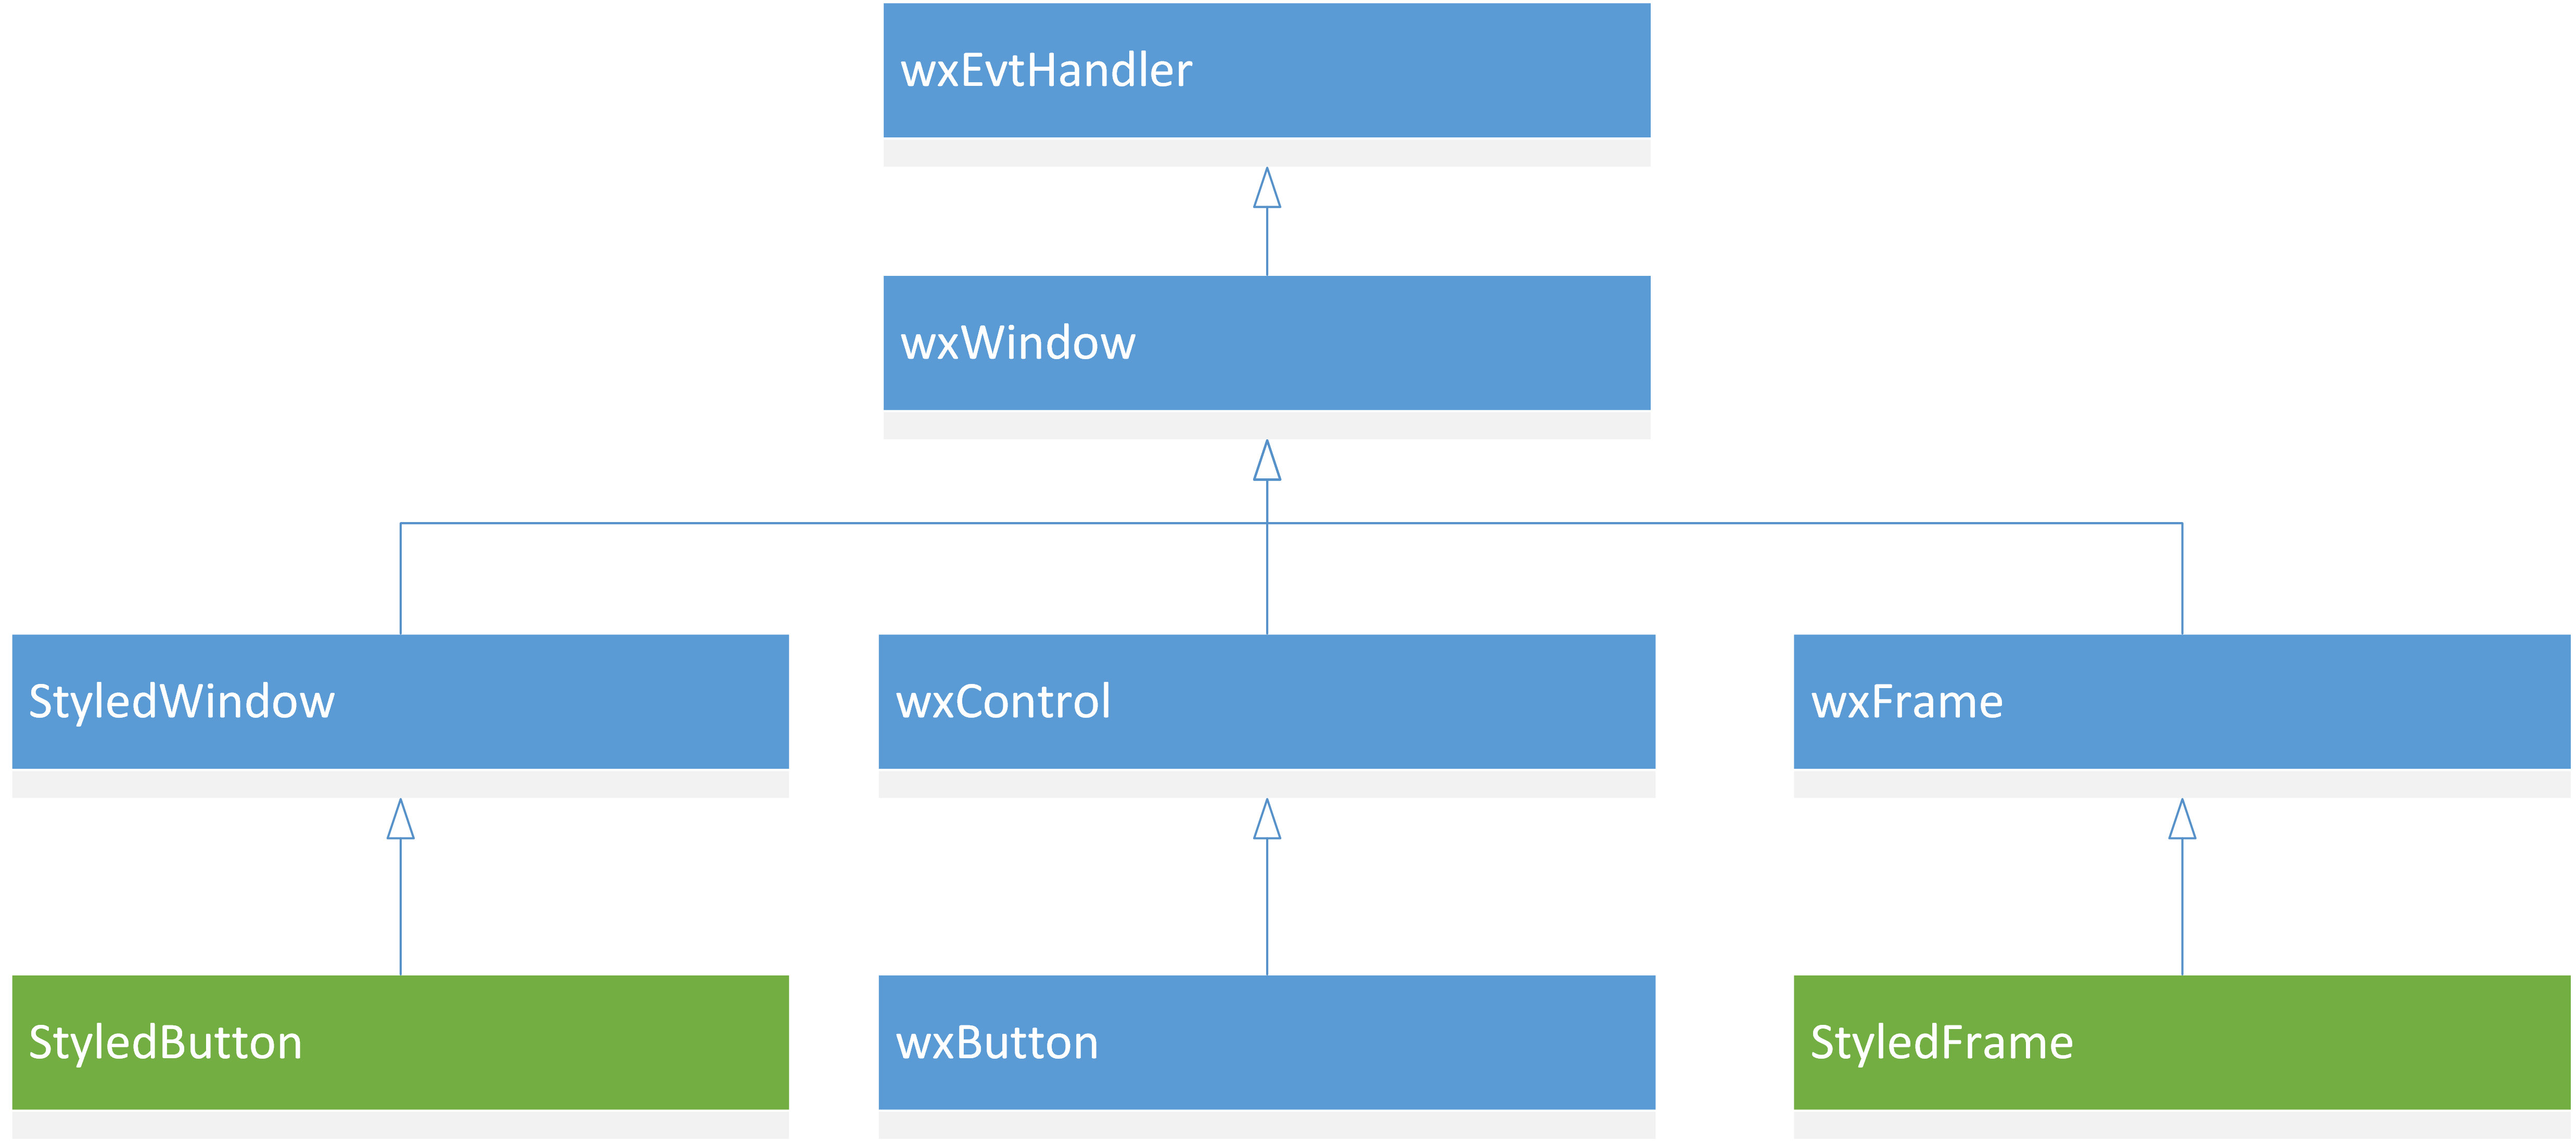
\includegraphics[scale=0.7]{img/ch5_class_system_architecture.png}
    \label{fig:ch5_class_system_architecture}
    \caption{Ierarhia de clase reprezentative pentru obiectele de interfa't'a ale bibliotecii wxStyle}
\end{figure}
\end{center}

Din nefericire mecanismul de procesare al evenimentelor implementat in wxWidgets nu permite legarea mai multor proceduri de procesare aceluia'si eveniment. Acest impediment este tratat 'in interiorul clasei StyledWindow folosind pattern-ul Observer 'in felul urmator:

\medskip

Clasa StyledWindow se conecteaz'a la toate evenimentele de interes pentru obiectele de interfa't'a din libr'aria wxStyle, cum ar fi evenimente de interac'tiune utilizator prin dispozitivul mouse sau tastatur'a, dar 'si evenimente de focus 'si desenare.
Clasa StyledWindow declar'a metode virtuale specializate pentru fiecare eveniment 'si care vor fi apelate 'in cazul intercept'arii evenimentului propriu-zis.
Clasa StyledWindow administreaz'a o list'a de obiecte de tip Listener: MouseListener, KeyboardListener, FocusListener and SizeListener. Aceste interfe'te declar'a metode de procesare a evenimentelor corespunz'atoare fiec'arei categorii. 'In urma apelului de metod'a virtual'a specializat'a pentru eveniment, clasa StyledWindow apeleaz'a metoda specializat'a din interiorul obiectelor de tip Listener care ii sunt ata'sate.

\medskip

[ diagrama UML de clase ]

\medskip

Tot 'in cadrul clasei StyledWindow se afl'a 'si suportul pentru stilizare 'si prezentare customizat'a (custom renderer). Acest lucru se face prin agregarea 'in cadrul clasei a unei instan'te de \emph{Style} 'si a uneia de \emph{StyledRenderer}. At{\ia}t clasele derivate dar 'si utilizatorii acestora pot folosi metode de tip Set 'si Get pentru a schimba instan'tele agregate. Pentru a implementa suportul pentru stilizare, clasa StyledWindow apeleaza medota de prezentare 'si desenare a instan'tei de StyledRenderer 'in cadrul proces'arii evenimentelor de tip Paint.

[ diagrama de comunicare ]

% ==============================================================================
%   Styled Frame
% ==============================================================================

\subsection{StyledFrame}

Obiectul de interfa't'a StyledFrame are rolul de a reprezenta o fereastr'a top-level. Ferestrele sunt compuse din:

\begin{itemize}
\item Cadrul 'si decora'tiunile de cadru care delimiteaz'a suprafa'ta ferestrei 'si permit redimensionarea acesteia.
\item Bara de titlu care con'tine icoana, titlul 'si ac'tiunile minimize, maximize 'si close ale ferestrei.
\item Zona de con'tinut unde sunt agregate obiectele de interfa't'a componente ale fiec'arei ferestre.
\end{itemize}

\begin{center}
\begin{figure}[H]
    \centering
    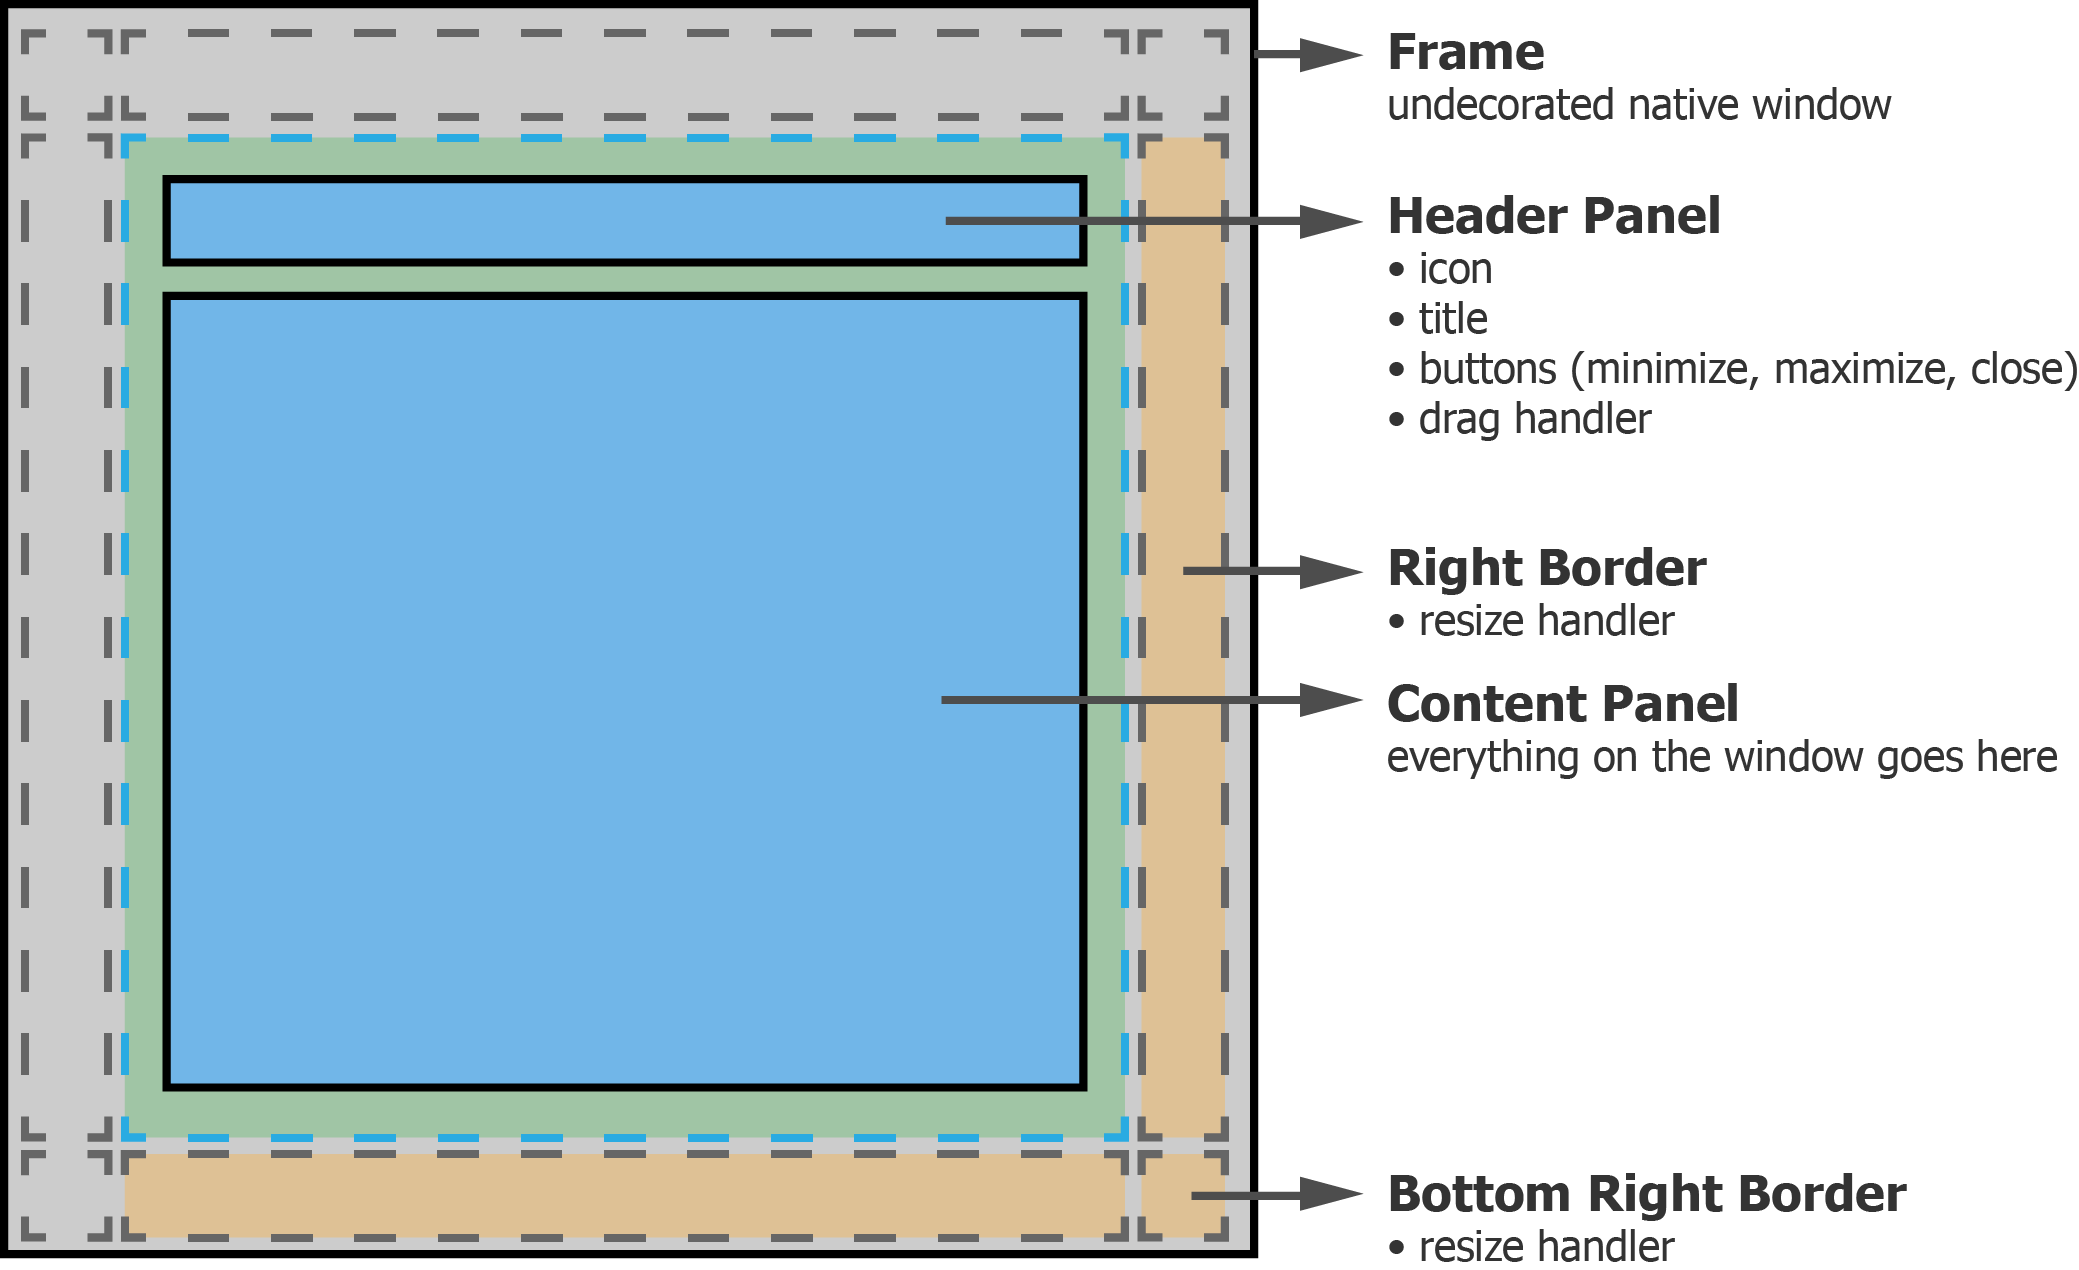
\includegraphics[scale=0.8]{img/ch5_styledframe.png}
    \label{fig:fig_5_2}
    \caption{Structura unei ferestre StyledFrame}
\end{figure}
\end{center}

Obiectul StyledFrame nu face parte din ierarhia de clase ce 'i'si are r'ad'acina 'in clasa StyledWindow deoarece o fereastr'a nu beneficiaz'a de acelea'si tr'as'aturi stilizabile comune celorlalte obiecte de interfa't'a. Aceasta este doar un container pentru ele. Mai mult, in cadrul ierarhiei wxWidgets, ferestrele sunt abstractizate prin clasa wxFrame care este mai specific'a decat wxWindow. Din acest motiv clasa p'arinte a clasei StyledFrame este wxWindow.

\medskip

Totu'si, ferestrele ar trebui s'a permit'a stilizare 'in privin'ta cadrului 'si a b'arii de titlul. Pentru a face acest lucru posibil, StyledFrame construie'ste o fereastr'a nativ'a nedecorat'a, adic'a o fereastr'a care nu con'tine cadru 'si bara de titlul. Pentru a oferii aceea'si func'tionalitate, 'in interiorul ferestrei nedecorate sunt ad'augate componente pentru cadru 'si titlul. 

\medskip

Cadrul este format din 8 panouri speciale distribuite pe marginile ferestrei care pot fi pictate individual pentru a construi orice aspect. La evenimentele de tip Mouse ale acestor panouri se ata'seaz'a componente speciale numite ResizeHandler. Aceste componente transform'a ac'tiunile de tip \emph{drag} ale panourilor de cadru 'in ac'tiuni de resize pentru fereastra p'arinte. 'In acest fel, panourile ce reprezint'a cadrul ferestrei 'indeplinesc 'si func'tionalitate de zone de redimensionare.

\medskip

Zona de titlu este reprezentat'a de o instan't'a a clasei FrameHeader. Aceast'a clas'a are rolul de a encapsula 'si implementa functionalitatea minim'a a unei b'ari de titlu cum ar fi: prezentarea icoanei, prezentarea titlului 'si prezentarea butoanelor de ac'tiune pentru fereastr'a. Mai mult, instan'ta acestei clase din cadru ferestrei poate fi schimbat'a, permi't{\ia}nd utilizatorului s'a construiasc'a ferestre cu b'ari de titlu customizabile 'si stilizabile. La evenimentele de tip Mouse ale acestei clase se ata'seaz'a o component'a de tip DragHandler. Aceast'a component'a are rolul de a interpreta ac'tiunile de tip \emph{drag} executate 'in interiorul zonei de titlu 'in evenimente de repozi'tionare a ferestrei.

\medskip

[ Diagrama UML cu toate clasele participante ]

% ==============================================================================
%   Styled Label
% ==============================================================================

\subsection{StyledLabel}

\begin{center}
\begin{figure}[h]
    \centering
    
\includegraphics{img/ch5_styledlabel.png}
    \label{fig:fig_5_1}
    \caption{O posibil'a reprezentare a unui obiect de interfa'ta StyledLabel}
\end{figure}
\end{center}



% ==============================================================================
%   Styled Button
% ==============================================================================

\subsection{StyledButton}

% ==============================================================================
%   Styled Checkbox
% ==============================================================================

\subsection{StyledCheckBox}

% ==============================================================================
%   Styled TextBox
% ==============================================================================

\subsection{StyledTextBox}

Capitolul de fa'ta are ca subiect implementarea obiectului de interfa't'a StyledTextBox ce permite introducerea 'si editarea de mesaje text. 

\begin{center}
\begin{figure}[h]
    \centering
    
\includegraphics{img/ch5_styledtextbox.png}
    \label{fig:fig_5_1}
    \caption{Editorul de text StyledTextBox}
\end{figure}
\end{center}

\medskip

Acest obiect este reprezentat de o c'asu't'a text 'si un cursor. 'In interiorul c'asu'tei text este prezentat mesajul introdus 'impreuna cu pozi'tia cursorului. De'si textul poate avea o lungime mai mare dec{\ia}t c'asu'ta ce 'il con'tine, caz 'in care va fi prezentat'a doar o parte a textului, cursorul trebuie s'a fie 'intotdeauna 'in interiorul c'asu'tei. Cursorul indica pozi'tia la care noile caractere vor fi introduse in mesajul text. Prin ad'augarea de caractere noi, cursorul i'si schimb'a pozi'tia.

\medskip

Tr'as'aturile 'si functionalitatea pe care un editor de text trebuie s'a le aib'a sunt:

\begin{itemize}
\item Introducerea de text prin ap'asarea tastelor ce reprezint'a caracterele mesajului sau prin alipirea de caractere salvate in \emph{Clipboard}.
\item Navigarea cursorului prin taste (st{\ia}nga, dreapta, home, end, etc.)
\item Navigarea cursorului prin mouse: ap'asarea butonului st{\ia}ng al mouse-ului deasupra textului deja introdus plaseaz'a cursorul 'in cea mai apropiat'a pozitie valid'a relativ la indicatorul mouse-ului.
\item Afi'sarea selectiv'a a textului astfel 'inc{\ia}t cursorul s'a fie 'intotdeauna 'in interiorul c'asu'tei text.
\item Selectarea textului prin taste sau prin mouse astfel 'inc{\ia}t cursorul s'a fie pozi'tionat 'intotdeauna la cap'atul selec'tiei.
\item Editarea textului selectat prin 'stergere sau 'inlocuire.
\item Posibilitatea revoc'arii ac'tiunilor prin func'tionalitate de tip \emph{undo} 'si \emph{redo}.
\end{itemize}

\medskip

Obiectul de interac'tiune implementat de libr'aria wxStyle implementeaz'a toate aceste tr'as'aturi, mai pu'tin posibilitatea anul'arii ac'tiunilor. Interac'tiunea cu utilizatorul se face prin interceptarea 'si interpretarea mesajelor generate de ac'tiunile utilizatorului precum: \emph{MouseMove}, \emph{MouseDown}, \emph{KeyPressed} 'si \emph{KeyChar}. Acestea sunt interceptate 'in super-clasa StyledWindow 'si pot fi procesate prin suprascrierea metodelor virtuale specifice fiec'arui mesaj.

\subsubsection{Introducere Text}

Introducerea textului se face prin inteceptarea mesajelor de tip \emph{KeyChar} care sunt transmise la ap'asarea unei taste ce reprezint'a un caracter vizibil ce nu a fost procesat prin interceptarea unui mesaj de tipul \emph{KeyPressed}.\footnote{http://docs.wxwidgets.org/3.0/classwx\_key\_event.html} Acest mesaj contine caracterul vizibil introdus 'si 'tine cont de starea tastelor \emph{CapsLock} respectiv \emph{Shift} care pot schimba caracterul reprezentat de celelalte taste.

\medskip

Caracterul con'tinut 'in mesaj este introdus 'in textul obiectului de interfa't'a la pozi'tia cursorului. Dac'a exist'a o selec'tie a textului in momentul introducerii caracterului, aceasta va fi inlocuit'a de noul caracter. 'In urma introducerii unui caracter, cursorul i'si schimb'a pozi'tia cu un caracter la dreapta, astfel inc{\ia}t noul caracter s' se afle in st{\ia}nga cursorlui. Dac' noua pozi'tie a cursorului 'il determin'a sa se afle in afara c'asu'tei de text, textul este mutat spre st{\ia}nga sau spre dreapta cu o distan'ta suficient de mare pentru a pozi'tiona cursorul la marginea st{\ia}ng'a respectiv dreapt'a a casu'tei text. Desenarea textului se face folosind un dreptunghi de t'aiere (clipping) care nu las'a textul ce nu se 'incadreaz'a in casu'ta de text, lu{\ia}nd 'in considerare marginile (insets), sa fie desenat.

\medskip

Introducerea textului prin alipire se face prin interceptarea mesajelor de tip \emph{\emph{KeyPressed}} ce descriu ap'asarea tastei \emph{V} 'impreun'a cu modificatorul \emph{Ctrl}.

\subsubsection{Navigare}

Navigarea prin taste se face prin interceptarea acelor mesaje de tip \emph{\emph{KeyPressed}} care au ca surs'a ap'asarea tastelor specifice navig'arii. Astfel, fiecare tasta predefinit'a determina repozi'tionarea cursorului la un nou index. Navigarea prin taste poate determina 'si terminarea selec'tiei printr-un eveniment de navigare ce nu modific'a selec'tia curent'a (ex. tasta \emph{Shift} nu apare ca modificator 'in compozi'tia evenimentului).

\medskip

Navigarea prin mouse se face intercept{\ia}nd acele mesaje de tip \emph{MouseDown} ce nu afecteaz'a starea de focus a obiectului. Prin ap'asarea butonului st{\ia}ng al mouse-ului se parcurge textul deja introdus pentru a g'asi index-ul al c'arui pozi'tie 'in spa'tiul c'asu'tei text este cel mai apropiat de pozi'tia indicatorului.

\subsubsection{Selec'tie}

Selec'tia este reprezentat'a de doi indexi: unul de 'inceput 'si unul de sf{\ia}r'sit. Indexul de 'inceput este 'intotdeauna ini'tializat la pozi'tia cursorului 'in momentul 'inceperii selec'tiei. Indexul de sf{\ia}r'sit este 'intotdeauna acela'si cu indexul cursorului. Modificarea selec'tiei se face 'in mod similar navig'arii normale. Dac'a evenimentul determin'a o schimbare in selec'tia curent'a, indexul de sf{\ia}r'sit al selec'tiei este actualizat la noua pozi'tie a cursorului. Din acest motiv, orice eveniment de navigare poate modifica selec'tia curent'a.

\medskip

'In momentul introducerii de text nou, fie prin alipire, fie prin modul standard, textul descris de selec'tia curent'a este eliminat. 'In acela'si fel, evenimentele de 'stergere ac'tioneaz'a mai 'int{\ia}i asupra selec'tiei curente dac'a exist'a, iar dac'a nu exist'a selec'tie, asupra caracterelor din vecin'atatea cursorului.

\medskip

Selec'tia 'intregului text este posibil'a prin procesarea mesajelor de tip \emph{KeyPressed} ce descriu ap'asarea tastei \emph{A} 'impreun'a cu modificatorul \emph{Ctrl}.

\subsubsection{Prezentare 'si desenare}

Prezentarea este implementat'a 'in cadrul prezentatorului implicit numit StyledTextBoxRenderer, care este privat implementat 'in sursa .cpp ce con'tine 'si implementarea obiectului de interfa'ta. Prezentatorul are rolul de a desena fundalul c'asu'tei text, textul, cursorul 'si selec'tia. Desenarea fundalului se face folosind instruc'tiunile de desenare specificate de stilul obiectului. Desenarea textului se face folosind descrierea de font specificat'a 'in stilul obiectului. Selec'tia 'si cursorul sunt desenate conform propriet'a'tilor SelectionColor 'si CursorWidth ale obiectului de interfa't'a.

\subsubsection{Dezvoltari ulterioare}

Obiectul de interfa't'a StyledTextBox implementeaz'a majoritatea tr'as'aturilor necesare unui editor de text, dar 'in acela'si timp 'ii lipsesc unele tr'as'aturi esen'tiale pentru a putea fi folosit confortabil. Printre aceste tr's'aturi ce lipsesc, amintim c{\ia}teva mai importante:

\begin{itemize}
\item Ac'tiuni de tipul \emph{undo} 'si \emph{undo} a acestui obiect de interfa'ta prin encapsularea ac'tiunilor 'in comenzi structurate 'intr-o stiv'a a istoricului.
\item Posibilitatea ascunderii textului pentru introducerea de informa'tie sensibil'a precum parole.
\item Posibilitatea filtr'arii caracterelor acceptate pentru a construi editoare de numere.
\end{itemize}

% ==============================================================================
%   Infrastructura
% ==============================================================================

\section{Infrastructur'a}

% ==============================================================================
%   Prezentare si desenare
% ==============================================================================

\section{Prezentarea 'si desenare obiectelor de interfa't'a}

Pentru a prezenta un obiect de interfa't'a, utiliz'am primitivele de desenare oferite de wxWidgets. Acestea sunt \emph{wxDC}\footnote{http://docs.wxwidgets.org/3.0/classwx\_d\_c.html} care reprezint'a un dispozitiv ce suport'a desenare 'si \emph{wxGraphicsContext}, o clas'a ce permite desenarea de obiecte grafice primitive pe suprafa'ta unui dispozitiv. 

\subsection{Dispozitive de desenare wxDC}

Un dispozitiv poate fi un fi'sier raster, un fi'sier vectorial, o imprimant'a sau suprafa'ta unei ferestre. Mai mult dec{\ia}t reprezentarea unei destina'tii pentru desenare, obiectele de tipul wxDC ofer'a 'si metode pentru desenarea efectiv'a. Pentru suprafa'ta unei ferestre, wxWidgets pune la dispozi'tie mai multe tipuri de DC-uri, precum \emph{wxClientDC}, \emph{wxWindowDC}, \emph{wxPaintDC}, \emph{wxBufferedPaintDC}, \emph{wxAutoBufferedPaintDC}.

\begin{itemize}
\item \textbf{wxWindowDC} ofer'a posibilitatea desen'arii pe 'intreaga suprafa't'a a unei ferestre, inclusiv marginile 'si decora'tiunile. Acest lucru este suportat doar pe sistemul de operare Windows.
\item \textbf{wxClientDC} ofer'a posibilitatea desen'arii 'in interiorul unei ferestre, 'in zona denumit'a zona client.
\item \textbf{wxPaintDC} este utilizat pentru a desena pe suprafa'ta client a unei ferestre 'in cadrul unei metode de procesare a evenimentului de desenare. Acest obiect are 'si rolul de a construi regiunea de clipping a ferestrei. wxWidgets necesit'a construirea unui astfel de obiect 'in interiorul metodei de procesare a evenimentelor de desenare, indiferent dac'a obiectul este folosit sau nu.
\item \textbf{wxBufferedPaintDC} este un device context de tipul \emph{buffered}, adic'a are suport pentru evitarea artefactelor de tipul \emph{flicker}. Este de asemenea un device context de tipul \emph{Paint}, adic'a poate fi folosit pentru a procesa evenimentele de desenare.
\item \textbf{wxAutoBufferedPaintDC} prezint'a o 'imbun'at'a'tire fa't'a de \emph{wxBufferedPaintDC} deoarece nu implementeaz'a procesul de double-buffering pe platformele care suport'a nativ acest lucru. Pentru a utiliza acest device context, este necesar specificarea stilului wxBG\_STYLE\_PAINT care previne procesul separat de desenare al fundalului.
\end{itemize}

'In urma test'arii fiec'arui tip de device context, cel mai potrivit s-a demonstrat a fi \emph{wxAutoBufferedPaintDC}. Acest lucru se datoreaz'a faptului ca elimina artefactele de tipul \emph{flicker} care sunt evidente 'si deranjante, 'in special 'in momentele 'in care un obiect de interfa't'a 'i'si schimb'a 'inf'a'ti'sarea datorit'a unei schimb'ari de stare. De asemenea, acest obiect este mai performant dec{\ia}t fratele s'au \emph{wxBufferedPaintDC}. Din nefericire, \emph{wxAutoBufferedPaintDC} presupune desenarea pe o suprafa't'a (imagine) intermediar'a, care este ini'tializat'a cu o culoare uniform'a neagr'a. Acest lucru previne posibilitatea de transparen't'a a obiectelor de interfa't'a. 

Lipsa de transparen'ta presupune imposibilitatea de desenare a unor obiecte de interfa't'a cu alte forme dec{\ia}t dreptunghiul care le delimiteaz'a. Un pas 'in rezolvarea acestei probleme a fost implementarea unui mecanism de g'asire a culorii de fundal 'in func'tie de ierarhia p'arin'tilor 'si proprietatea de transparen't'a a acestora. Algoritmul recursiv este urm'atorul:

\begin{enumerate}
\item Dac'a obiectul este opac, utilizeaz'a culoarea de fundal a obiectului.
\item Dac'a obiectul este transparent:
	\begin{enumerate}
	\item Dac'a are p'arinte, utilizeaz'a culoarea de fundal a parintelui.
	\item Dac'a nu are p'arinte, itlizeaz'a o culoare predefinit'a (negru).
	\end{enumerate}
\end{enumerate}

Acest algoritm nu func'tioneaz'a dac'a vreunul dintre p'arin'ti utilizeaz'a unul din procesele de stilizare 'si prezentare puse la dispozi'tie de biblioteca wxStyle. 'In schimb, este util pentru cazul simplu 'in care obiectele de interfa't'a sunt 'incadrate 'intr-o fereastr'a cu un fundal umplut cu o culoare uniform'a.

\subsection{Mecanismul de desenare wxGraphicsContext}

Pentru a acomoda evolu'tia API-urilor pentru desenare grafic'a, wxWidgets a introdus un nou mecanism de desenare prin obiecte de tipul \emph{wxGraphicsContext}. Aceste obiecte sunt construite printr-un \emph{wxRenderer} care reprezint'a unul din API-urile grafice abstractizate de wxWidgets. Printre aceste API-uri, pe platforma Windows sunt disponibile \emph{Cairo}, \emph{GDI+} 'si, mai nou, \emph{Direct2D}. Obiectele de tipul \emph{wxGraphicsContext} sunt ata'sate unui dispozitiv la momentul construc'tiei.

\medskip

Diferit fa't'a de API-ul pentru desenare oferit de obiectele \emph{wxDC}, \emph{wxGraphicsContext} lucreaz'a cu obiecte speciale numite \emph{wxGraphicsObjects} care descriu pensule, peni'te, traiectorii 'si matrici de transfomare. Aceste obiecte encapsuleaz'a 'si abstractizeaz'a obiectele native ale API-ului grafic, 'si fac leg'atura cu obiectele specializate wxWidgets precum \emph{wxPen}, \emph{wxBrush}, etc.

\medskip

Prezentatorii din biblioteca wxStyle folosesc obiecte de tipul wxGraphicsContext pentru a executa instruc'tiunile de desenare. Un exemplu de cod care ini'tializeaz'a un context de desenare pentru a fi folosit in interiorul unei metode de prezentare este prezent in figura \ref{fig0510}. Pentru a asigura dealocarea corect'a 'si distrugerea obiectului de tipul \emph{wxGraphicsContext*}, utiliz'am un pointer inteligent din libr'aria standard C++.

\begin{figure}[H]
\begin{lstlisting}[language=C++]
// g is a pointer to a wxGraphicsContext which is 
// automatically destroyed at the end of the method
wxAutoBufferedPaintDC dc(label);
auto g = unique_ptr<wxGraphicsContext>(wxGraphicsContext::Create(dc)).get();
\end{lstlisting}
\caption{Exemplu de ini'tializare al unui wxGraphicsContext}
\label{fig0510}
\end{figure}
%
%% ==============================================================================
%%   Capitolul 6: Testare si validare
%% ==============================================================================
%
\chapter{Testare}
\pagestyle{headings}

Pentru testarea bibliotecii wxStyle, a'sa cum este cazul cu toate proiectele software, recunoa'stem trei tipuri de testare ce difer'a at{\ia}t prin aria pe care o acoper'a c{\ia}t 'si elementele care sunt testate. Aceste tipuri sunt:

\begin{enumerate}
\item Testarea la nivel de cod - presupune testarea individual'a a componentelor individuale ce alc'atuiesc sistemul 'si formeaz'a infrastructura acestuia. Aceste teste sunt func'tionale 'si trateaz'a componentele ca pe ni'ste cutii negre ale c'aror implementare este irelevant'a. Testele de acest tip sunt automate, ceea ce 'inseamn'a ca pot detecta bug-uri recurente (regression testing) 'si se poate realiza o testare global'a a 'intregului sistem la orice nou' a modificare. Metodologia \emph{Test Driven Development} descrie un proces numit \emph{Red, Green, Refactor} care presupune 'inceperea proiectului prin scrierea de teste ce descriu 'si verific'a func'tionalitatea proiectului. Deoarece aceste teste sunt scrise 'inaintea implement'arii, ele vor pica, adic'a vor fi \emph{Red}. Urm'atorul pas este implementarea func'tionalit'a'tii care determin'a trecerea tuturor testelor, fac{\ia}ndu-le \emph{Green}. Pentru a asigura un cod curat si bine 'intre'tinut, ultimul pas presupune cur'a'tarea 'si rafinarea acestuia prin procesul de \emph{Refactoring}.
\item Testarea la nivel de bibliotec'a - presupune testarea func'tionalit'a'tii 'intregului sistem al bibliotecii. Aceste teste pot fi implementate similar cu cele de la nivelul de cod, dac'a sistemul permite testarea sub form'a de cutie neagr'a.
\item Testarea la nivel de aplica'tie - presupune testarea func'tionalit'a'tii aplica'tiei, presupun{\ia}nd c'a aceasta este alc'atuit'a din componente testate. O aplica'tie ce utilizeaz'a biblioteca wxStyle este implicit o aplica'tie cu interfa't'a vizual'a. Testarea unei astfel de aplica'tii necesit'a simularea interac'tiunii cu utilizatorul 'si interpret'arii rezultatelor afi'sate. De'si exist'a framework-uri ce realizeaz'a aceast'a func'tionalitate pentru biblioteci de interfa't'a precum Java Swing \footnote{https://code.google.com/p/fest/}, biblioteca wxWidgets nu beneficiaz'a de astfel de unelte, iar implementarea lor este una deosebit de dificil'a.\cite{tdddoesntwork}
\end{enumerate}

Scopul proiectului este acela de a realiza o bibliotec'a de obiecte vizuale stilizabile, deci testele la nivel de aplica'tie nu se aplic'a 'in acest context.

\section{Testare la nivel de cod}

Pentru testarea la nivel de cod am utilizat biblioteca \emph{boost::test} pentru a construi unit teste automate, grupate in suite. Spre deosebire de metodologia \emph{Test Driven Development}, am scris testele 'in urma scrierii codului. Testele sunt implementate in proiectul numit \emph{tests} care face parte din solu'tia Visual Studio a proiectului. Un exemplu de test scris cu ajutorul bibliotecii \emph{boost::test} 'il g'asi'ti in figura \ref{fig0601}

\begin{figure}[H]
\begin{lstlisting}[language=C++]
BOOST_AUTO_TEST_CASE(style_loading) {
    XMLStylesheetLoader loader;
    Stylesheet stylesheet = loader.Load("test.xml");
    DefinitionBundle defaultStyle = stylesheet.GetStyle("default").GetBundle(Style::CAT_DEFAULT);
    BOOST_CHECK(defaultStyle.GetBackgroundColor() == "#323335");
}
\end{lstlisting}
\caption{Exemplu de testare al unei componente utiliz{\ia}nd biblioteca \emph{boost::test}}
\label{fig0601}
\end{figure}

Testele din proiectul \emph{tests} acoper'a urm'atoarele componente ale bibliotecii wxStyle:

\begin{itemize}
\item Defini'tiile de stil - sunt testate folosind mijloacele de construire prin cod, iar apoi valorile lor sunt verificate s'a fie egale cu valorile folosite la construire. Se mai testeaz'a 'si opera'tia de combinare (merge) a mai multor defini'tii de stil.
\item Structura \emph{Unified Dimension} - este testat'a prin verificarea valorii calculate din componentele relative 'si absolute este corect'a relativ la o valoare de referin't'a. De asemenea, este testat'a parsarea corect'a a valorilor din reprezentarea de tip string, adic'a a metodei \emph{Dimension::ValueOf(std::string)}. Testele acestei structuri verific'a 'si corectitudinea structurilor \emph{DimPoint} 'si \emph{DimRect}.
\item 'Inc'arcarea fi'sierelor de stiluri - este testat'a verific{\ia}nd rezultatul produs de metoda \emph{XMLStylesheetLoader} asupra unui fi'sier de stiluri de test.
\item 'Inc'arcarea 'si adiministrarea imaginilor - este testat'a utiliz{\ia}nd imagini de test care sunt 'inc'arcate prin clasa \emph{ImageRepository}.
\item Algoritmi - precum calculul offset-ului utiliz{\ia}nd ancore verticale si orizontale sunt testa'ti aplic{\ia}nd algoritmii pe valori predefinite, iar apoi verific{\ia}nd rezultatul acestora 'impotriva rezultatelor a'steptate.
\item Instruc'tiunile de desenare - sunt testate doar prin construc'tia acestora 'si verificarea parametrilor.
\end{itemize}

\section{Testare la nivel de bibliotec'a}

Testarea la nivel de bibliotec'a presupune testarea obiectelor de interfa't'a at{\ia}t din punct de vedere al func'tionalit'a'tii acestora, dar 'si din punct de vedere al prezent'arii lor. Pentru a testa func'tionalitatea obiectelor de interfa't'a, trebuie sa simulam evenimentele produse de utilizator 'si s'a observ'am schimb'arile in starea componentelor 'si evenimentele generate de acestea. Pentru a testa modul de prezentare al obiectelor de interfa't'a, trebuie sa compar'am figura grafic'a a obiectului de interfa't'a cu figura a'steptat'a. Pentru a automatiza ambele moduri de testare presupune efort sporit si investi'tie de timp pe care nu l-am putut aloca. Din acest motiv, testarea la nivel de bibliotec'a se realizeaz'a utiliz{\ia}nd aplica'tia demonstrativ'a.

\begin{figure}[H]
\begin{center}
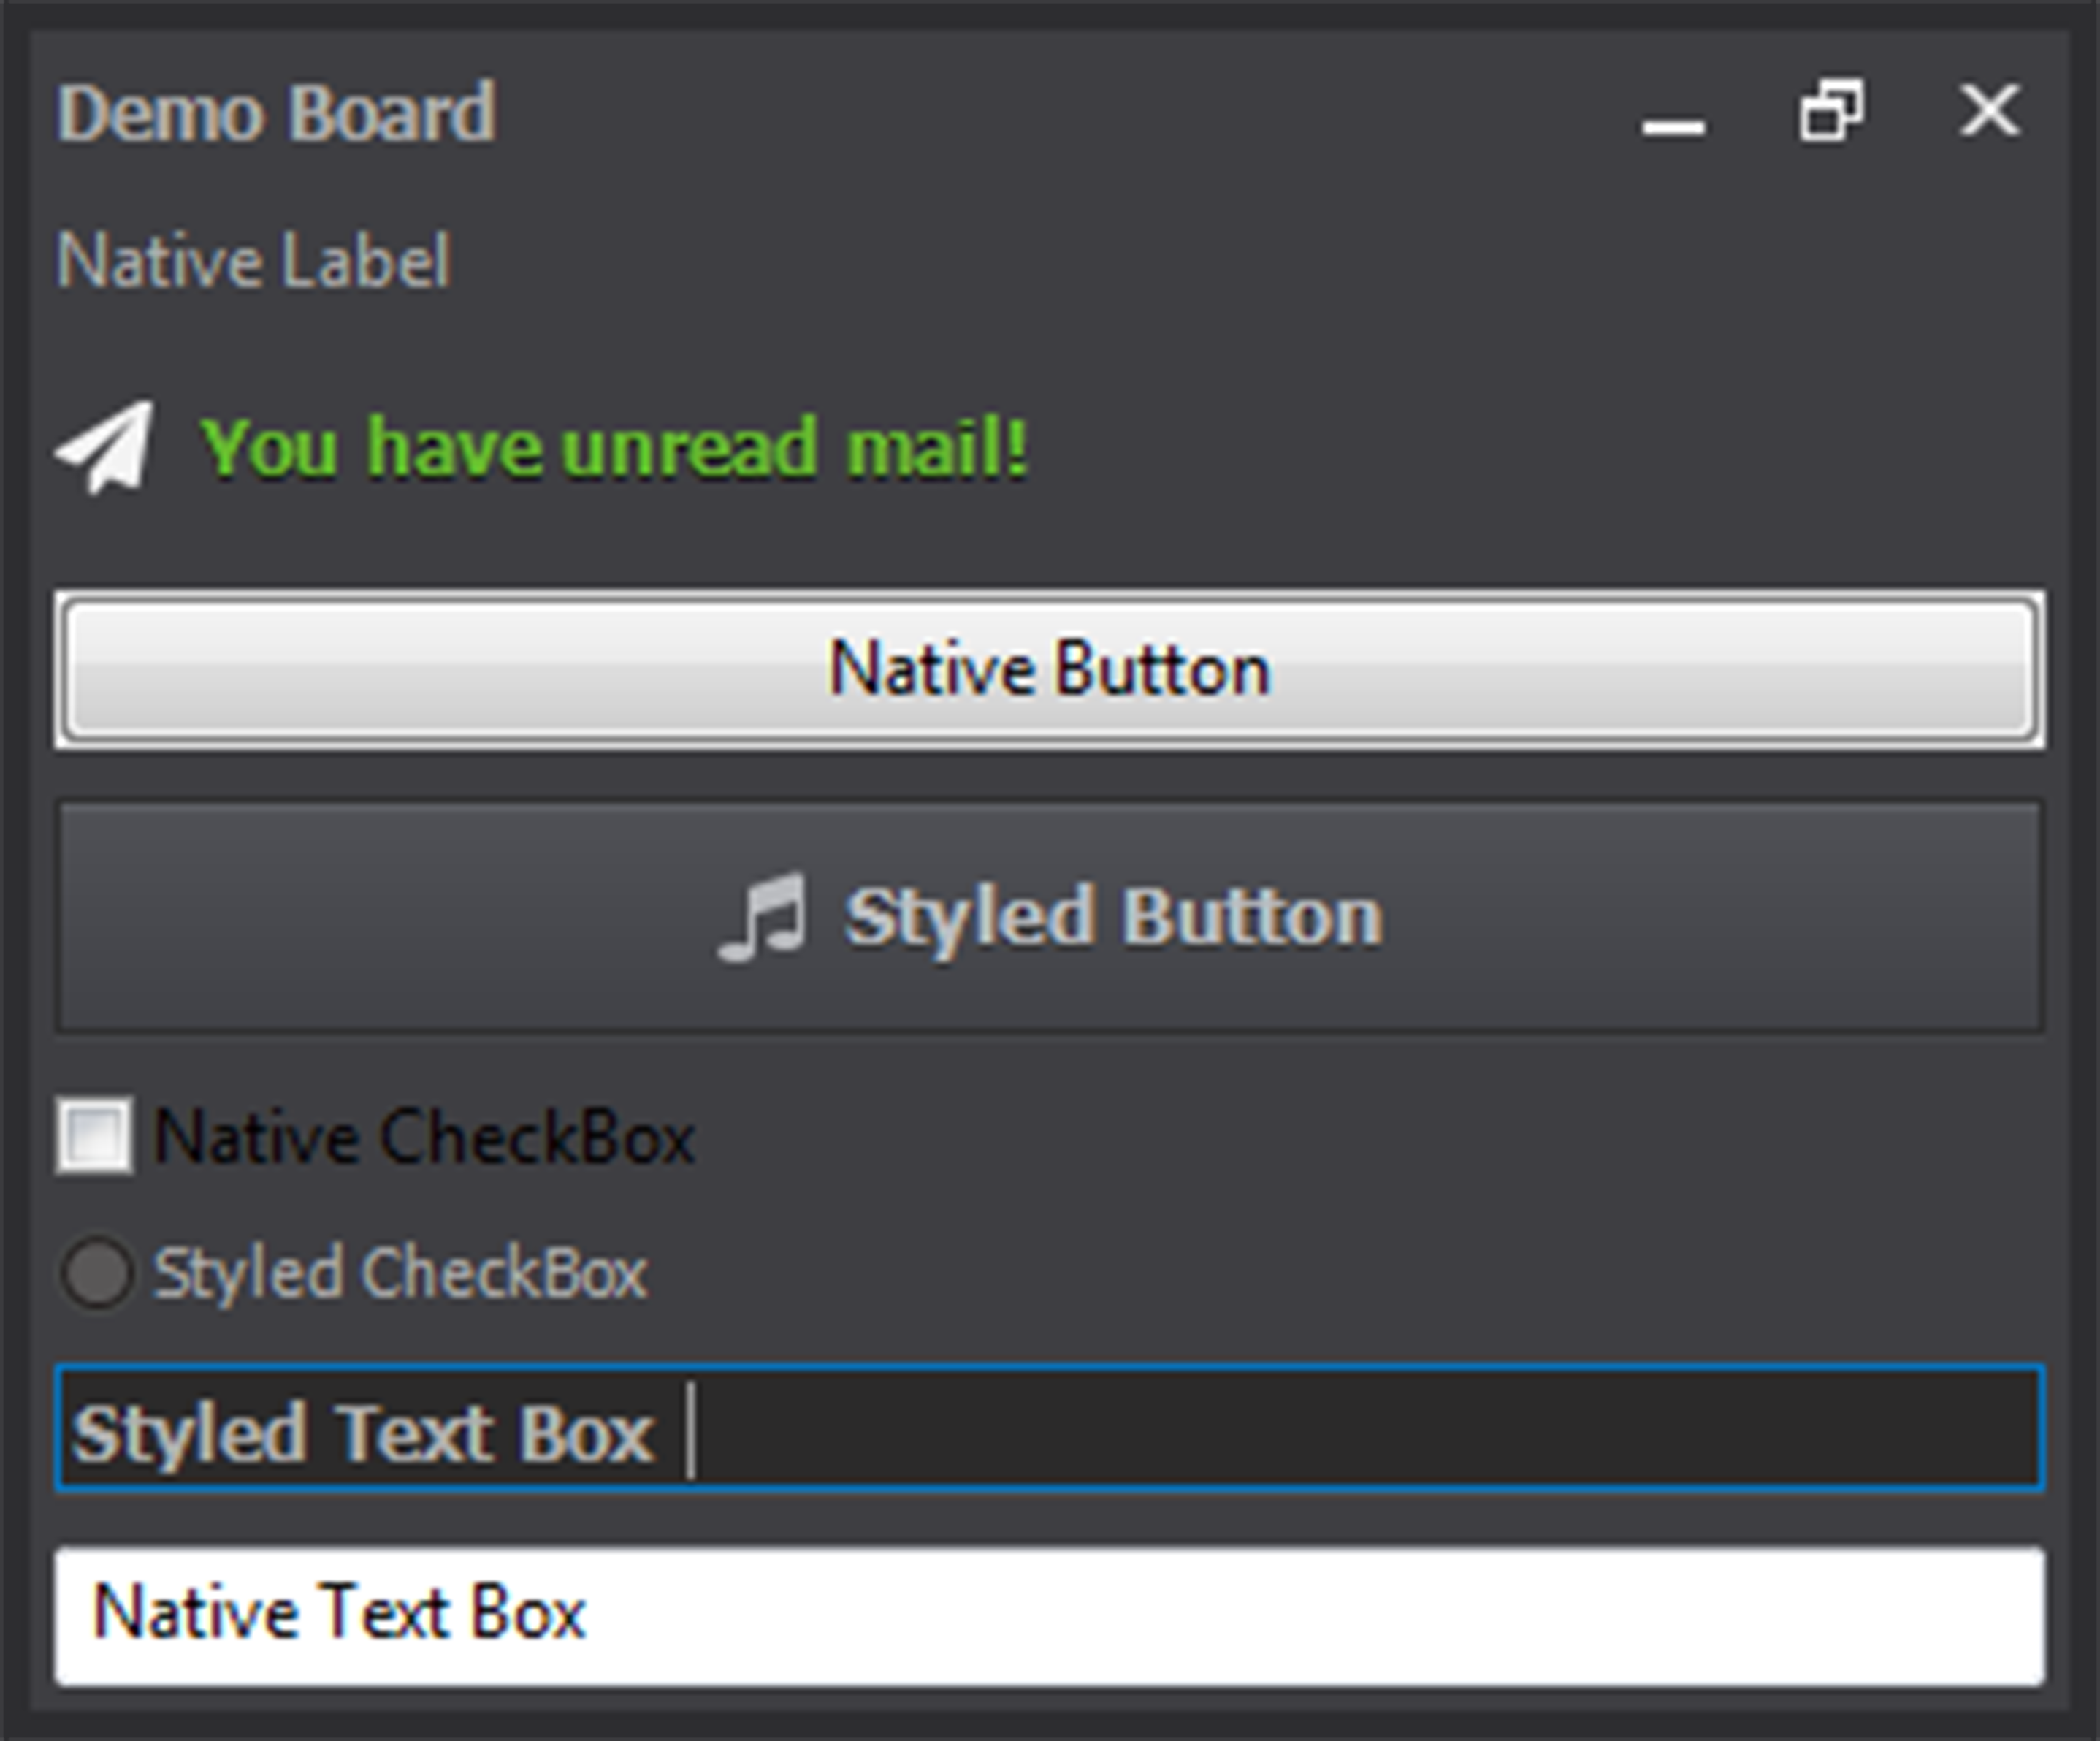
\includegraphics{img/ch6_demo_app.png}
\end{center}
\caption{Captur'a de ecran a aplica'tiei demonstrative}
\label{fig0602}
\end{figure}

Aplica'tia demonstrativ'a con'tine obiecte de interfa't'a stilizabile dar 'si obiecte de interfa't'a din biblioteca wxWidgets. Acestea din urm'a sunt prezente pentru a putea face o compara'tie 'intre modul de prezentare 'si func'tionare al obiectelor stilizabile. Figura \ref{fig0602} prezint'a o captur'a de ecran a aplica'tiei demonstrative.

\medskip

Aplica'tia demonstrativ'a permite urm'atoarele teste:

\begin{itemize}
\item Testarea ferestrei prin posibilitatea de redimensionare 'si mi'scare. Se poate testa manual comportamentul ramei ferestrei, butoanelor de ac'tiune precum minimize, maximize 'si close, 'si aspectul panoului de titlu. Se mai poate testa manual comportamentul panoului de titlu la ac'tiuni de tipul \emph{drag} care trebuie s'a determine mi'scarea ferestrei.
\item Testarea func'tionalit'a'tii obiectelor de interfa't'a. La obiectele de interfa't'a se ata'seaz'a observatori de evenimente care notific'a printr-un dialog de mesaj producerea unui eveniment. 'In acest fel, evenimentele generate de obiectele de interfa't'a sunt semnalate utilizatorului. Se mai poate testa comportamentul acestora la evenimente de intrare precum mi'scarea dispozitivului mouse, ap'as'area de butoane 'si taste, etc. De exemplu, pentur obiectul de interfa't'a StyledTextBox poate fi testat comportamentul la introducerea unui text mai lung dec{\ia}t cutia de text, sele'ctia folosind tastele de navigare, rezultatul ac'tiunilor de stergere asupra unui text vid, etc.
\item Testarea prezent'arii obiectelor de interfa't'a. Prin specificarea, 'in cadrul aplica'tiei demonstrative, unor stiluri, utilizatorul poate verifica modul de prezentare al obiectelor de interfa't'a. Acesta (utilizatorul) poate observa reprezent'arile diferite ale unui obiect 'in func'tie de starea acestuia. De exemplu: modul de prezentare al butonului c{\ia}nd este l'asat liber, c{\ia}nd este acoperit de dispozitivul mouse, c{\ia}nd este ap'asat, etc.
\end{itemize}

De'si mai pu'tin puternic'a dec{\ia}t o alternativ'a automat'a, testarea manual'a utiliz{\ia}nd aplica'tia demonstrativ'a ofer'a posibilitatea compara'tiei 'intre obiectele native wxWidgets, considerate a fi standard, 'si cele stilizabile. Mai mult dec{\ia}t o alternativ'a automat'a, o astfel de testare ii ofer'a utilizatorului posibilitatea test'arii oric{\ia}tor scenarii, intr-un mediu real (fa't'a de unul simulat). O astfel de testare manual'a permite observarea laten'tei 'si a timpului de r'aspuns 'si a artefactelor de desenare. Cu toate acestea este de dorit implementarea unui framework de testare automat'a, pentru a asigura func'tionalitatea corect'a a tuturor elementelor de interfa't'a, f'ar'a a irosi timp de testare manual'a.
%
%% ==============================================================================
%%   Capitolul 7: Manual de Instalare si Utilizare
%% ==============================================================================
%
\chapter{Manual de Instalare 'si Utilizare}
\pagestyle{headings}

\section{Cerin'te}

'In acest capitol sunt prezentate cerin'tele software si hardware necesare compil'arii 'si utiliz'arii libr'ariei wxStyle.

\subsection{wxWidgets}

Pentru a compila 'si utiliza libr'aria wxStyle, trebuie s'a ave'ti la dispozi'tie fi'sierele binare redistribuite ale libr'ariei wxWidgets. Pute'ti ob'tine aceste fi'siere fie 'in urma compil'arii libr'ariei, fie desc'arc{\ia}nd de pe internet o versiune compilat'a a acesteia. At{\ia}t sursele libr'ariei c{\ia}t 'si versiunea compilat'a a acesteia pot fi downloadate gratuit de la adresa oficial'a\footnote{http://wxwidgets.org/downloads/}.

\subsection{boost}

Libr'aria boost pentru C++ poate fi downloadat'a gratuit de la adresa oficial'a\footnote{http://www.boost.org/users/download/}. Pute'ti alege sa downloada'ti fie sursele libr'ariei, fie o versiune precompilat'a. Dac'a alege'ti sa downloada'ti sursele, urma'ti pa'sii de instalare detalia'ti 'in documentul de utilizare al libr'ariei disponibil online\footnote{http://www.boost.org/doc/libs/1\_55\_0/more/getting\_started/}.

\subsection{Sistem de operare}

Pentru a func'tiona corect, wxStyle are nevoie de un sistem de operare pentru care wxWidgets s'a implementeze mecanismul avansat de desenare. Sistemele de operare suportate sunt: 
\begin{itemize}
\item \textbf{Windows:} Windows XP, Windows Vista, Windows 7, Windows 8, Windows 8.1 
\item \textbf{Unix:} Aproape toate implementarile Unix 'impreun'a cu un cel pu'tin un desktop manager la alegere dintre: GTK+ 1.2, GTK+ 2.0, Motif 1.2 sau mai nou, Lesstif.
\item \textbf{MacOS:} Mac OS 8.6/9.x (ex. Classic) sau Mac OS X 10.x. 
\end{itemize}

\subsection{Compilator}

Libr'aria wxStyle utilizeaz'a c{\ia}teva dintre noile adi'tii la standardul C++ introduse 'in versiunea numit'a C++11. Din acest motiv, compilarea libr'ariei necesit'a un compilator ce implementeaz'a aceste tr'as'aturi. Majoritatea compilatoarelor moderne implementeaz'a aproape 'in 'intregime standardul C++11 'si sunt potrivite pentru compilarea proiectului. Dintre acestea men'tion'am: Visual Studio 2012, Visual Studio 2013 'si gcc 4.9.0. Orice compilator a'ti alege, este recomandat'a folosirea celei mai noi versiuni pentru a asigura nu doar compatibilitatea cu standardul, dar 'si cele mai bune performan'te 'si securitate.

\section{Compilare 'si Instalare}

Toate fisierele necesare configur'arii 'si compil'arii proiectului se afl'a 'in folder-ul \texttt{build}. Pentru compilarea libr'ariei se folose'ste un mecanism automat de generare a fi'sierelor proiect pentru editorul integrat Visual Studio. Acestea se genereaz'a pe baza unui script lua numit \texttt{premale4.lua}, prin rularea script-ului bash \texttt{update\_build.bat}. 'Inainte de generarea proiectului, asigura'ti-v'a c'a fi'sierul \texttt{paths.lua} con'tine c'aile corecte c'atre libr'ariile wxWidgets 'si boost.

Fi'sierul \texttt{paths.lua} con'tine dou'a variabile ce trebuiesc asignate: \texttt{SYSTEM\_LIBS} 'si \texttt{BOOST\_LIBS}. La calea specificat'a de variabila \texttt{SYSTEM\_LIBS} trebuie s'a se g'aseasc'a dou'a foldere: 
\begin{itemize}
\item \texttt{include} care s'a con'tin'a con'tinutul folder-ul \texttt{include} din libr'aria wxWidgets
\item \texttt{lib} care s'a con'tin'a toate fi'sierele .lib compilate ale libr'ariei wxWidgets
\end{itemize}

Calea specificat'a de \texttt{SYSTEM\_LIBS} trebuie sa con'tin'a libr'aria boost compilat'a.

Pentru generarea proiectului Visual Studio, executati scriptul \texttt{update\_build.bat}. In urma execu'tiei trebuie s'a rezulte folder-ul \texttt{vc2012} ce con'tine, printre altele, proiectul \texttt{wxstyle.sln}. Deschide-'ti acest proiect in editorul integrat Visual Studio 2012. Proiectul ar trebui s'a arate similar cu cel din figura urm'atoare:

% =================================
% Figura Proiect Visual Studio
% =================================
\begin{figure}[H]
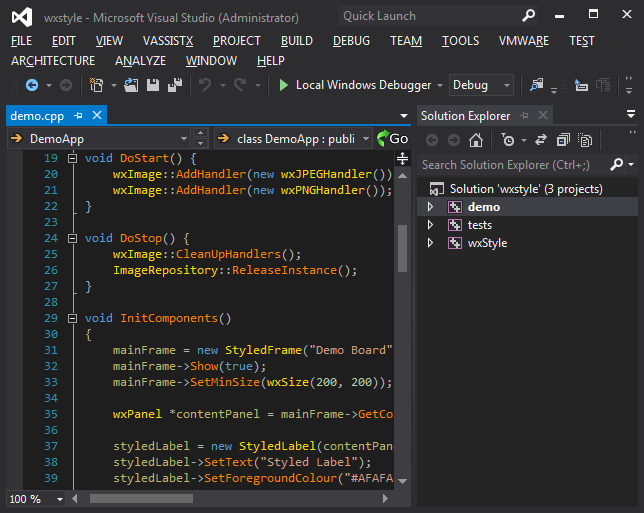
\includegraphics[width=15cm]{img/ch7_project.png}
\caption{Proiectul Visual Studio}
\label{fig:figure6.1}
\end{figure}

Pentru a compila libr'aria, este suficient s'a da'ti click dreapta pe numele proiectului wxStyle si alege'ti ac'tiunea Build. Proiectul este configurat sa compileze o librarie static'a, iar rezultatul compil'arii se poate gasi in folderul \texttt{lib}. Modul implicit de compilare este cel Debug, rezult{\ia}nd 'in libr'aria static'a \texttt{wxstyle\_d.lib} care con'tine 'si simboluri pentru depanare. Dac'a se alege din Visual Studio modul de compilare Release, rezultatul va fi \texttt{wxstyle.lib}.

Solu'tia con'tine de asemenea un proiect pentru testarea componentelor numit \texttt{tests} si un proiect demonstrativ ce prezint'a componentele libr'ariei wxStyle.


\section{Utilizare}

Aceast'a sec'tiune presupune c'a de'tine'ti o versiune compilat'a a libr'ariei dup'a ce a'ti urmat pa'sii din sec'tiunea anterioar'a. De asemenea, aceast'a sec'tiune presupune c'a ave'ti disponibil'a o versiune a editorului integrat Visual Studio 2012.

\subsection{Preg'atire}

Pentru a putea utiliza biblioteca wxStyle, trebuie s'a configura'ti 'in prealabil editorul Visual Studio 2012. Acest lucru presupune specificarea c'aii catre fi'sierele header ale bibliotecii, si a fisierului binar \emph{wxstyle.lib}.

\begin{enumerate}
\item Executa'ti click dreapta pe numele proiectului 'si alege'ti op'tiunea Properties.
\item La categoria \emph{C/C++}, subcategoria \emph{General} completa'ti c{\ia}mpul \emph{Additional Include Directories} cu calea relativ'a sau absolut'a c'atre folder-ul \emph{include} al bibliotecii wxStyle (vezi figura \ref{ch7_ide_include}).
\item La categoria \emph{Linker}, subcategoria \emph{General} completa'ti c{\ia}mpul \emph{Additional Library Directires} cu calea relativ'a sau absolut'a c'atre folder-ul \emph{lib} al bibliotecii wxStyle. In acest folder trebuie s'a existe fi'sierul compilat \emph{wxstyle.lib} (vezi figura \ref{ch7_ide_lib_folder})
\item La categoria \emph{Linker}, subcategoria \emph{Input} completa'ti c{\ia}mpul \emph{Additional Dependencies} cu numele fi'sierului binar al libr'ariei, mai exact \emph{wxstyle.lib} (vezi figura \ref{ch7_ide_lib_file}).
\end{enumerate}

\begin{figure}[H]
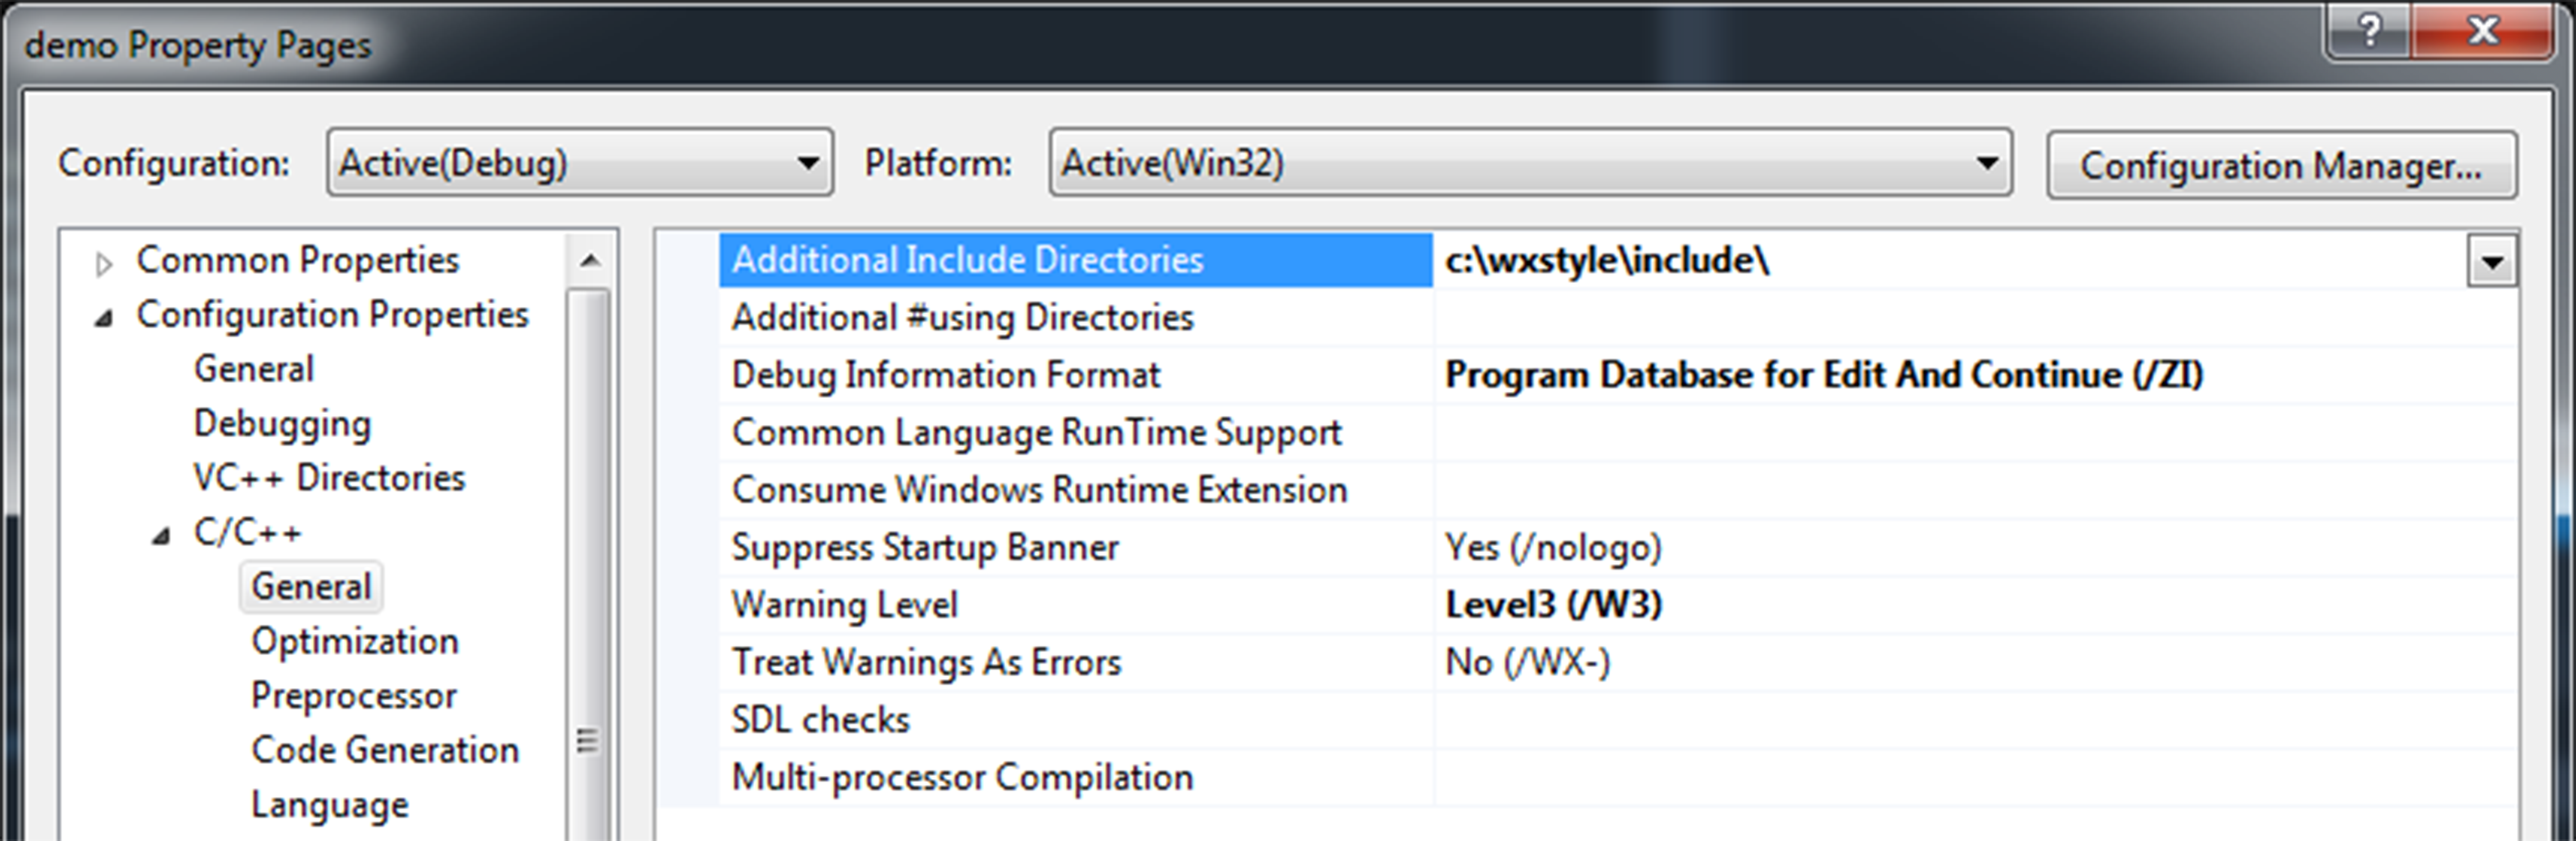
\includegraphics[width=15cm]{img/ch7_ide_include.png}
\caption{Setarea c'aii c'atre headerele bibliotecii wxStyle}
\label{ch7_ide_include}
\end{figure}

\begin{figure}[H]
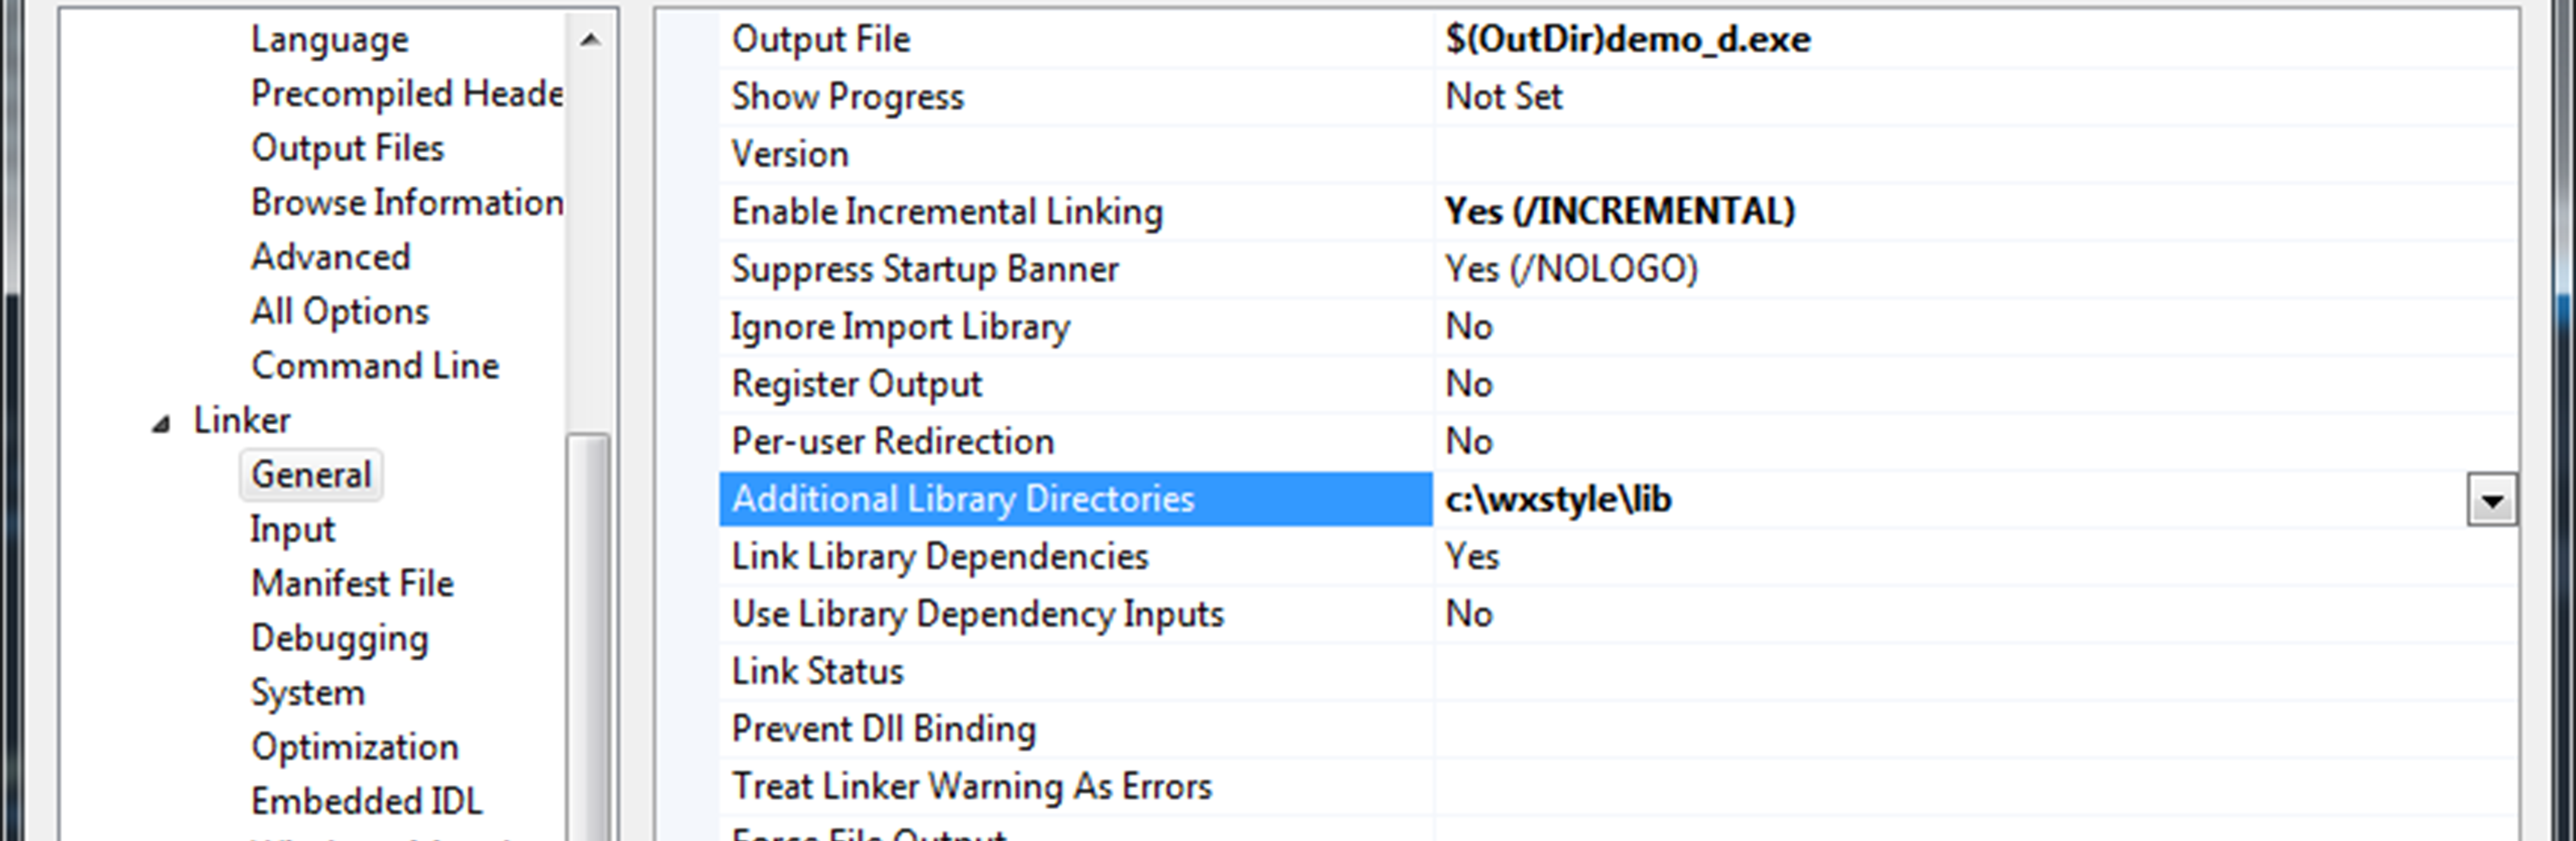
\includegraphics[width=15cm]{img/ch7_ide_lib_folder.png}
\caption{Setarea c'aii c'atre fi'sierul binar al bibliotecii wxStyle}
\label{ch7_ide_lib_folder}
\end{figure}

\begin{figure}[H]
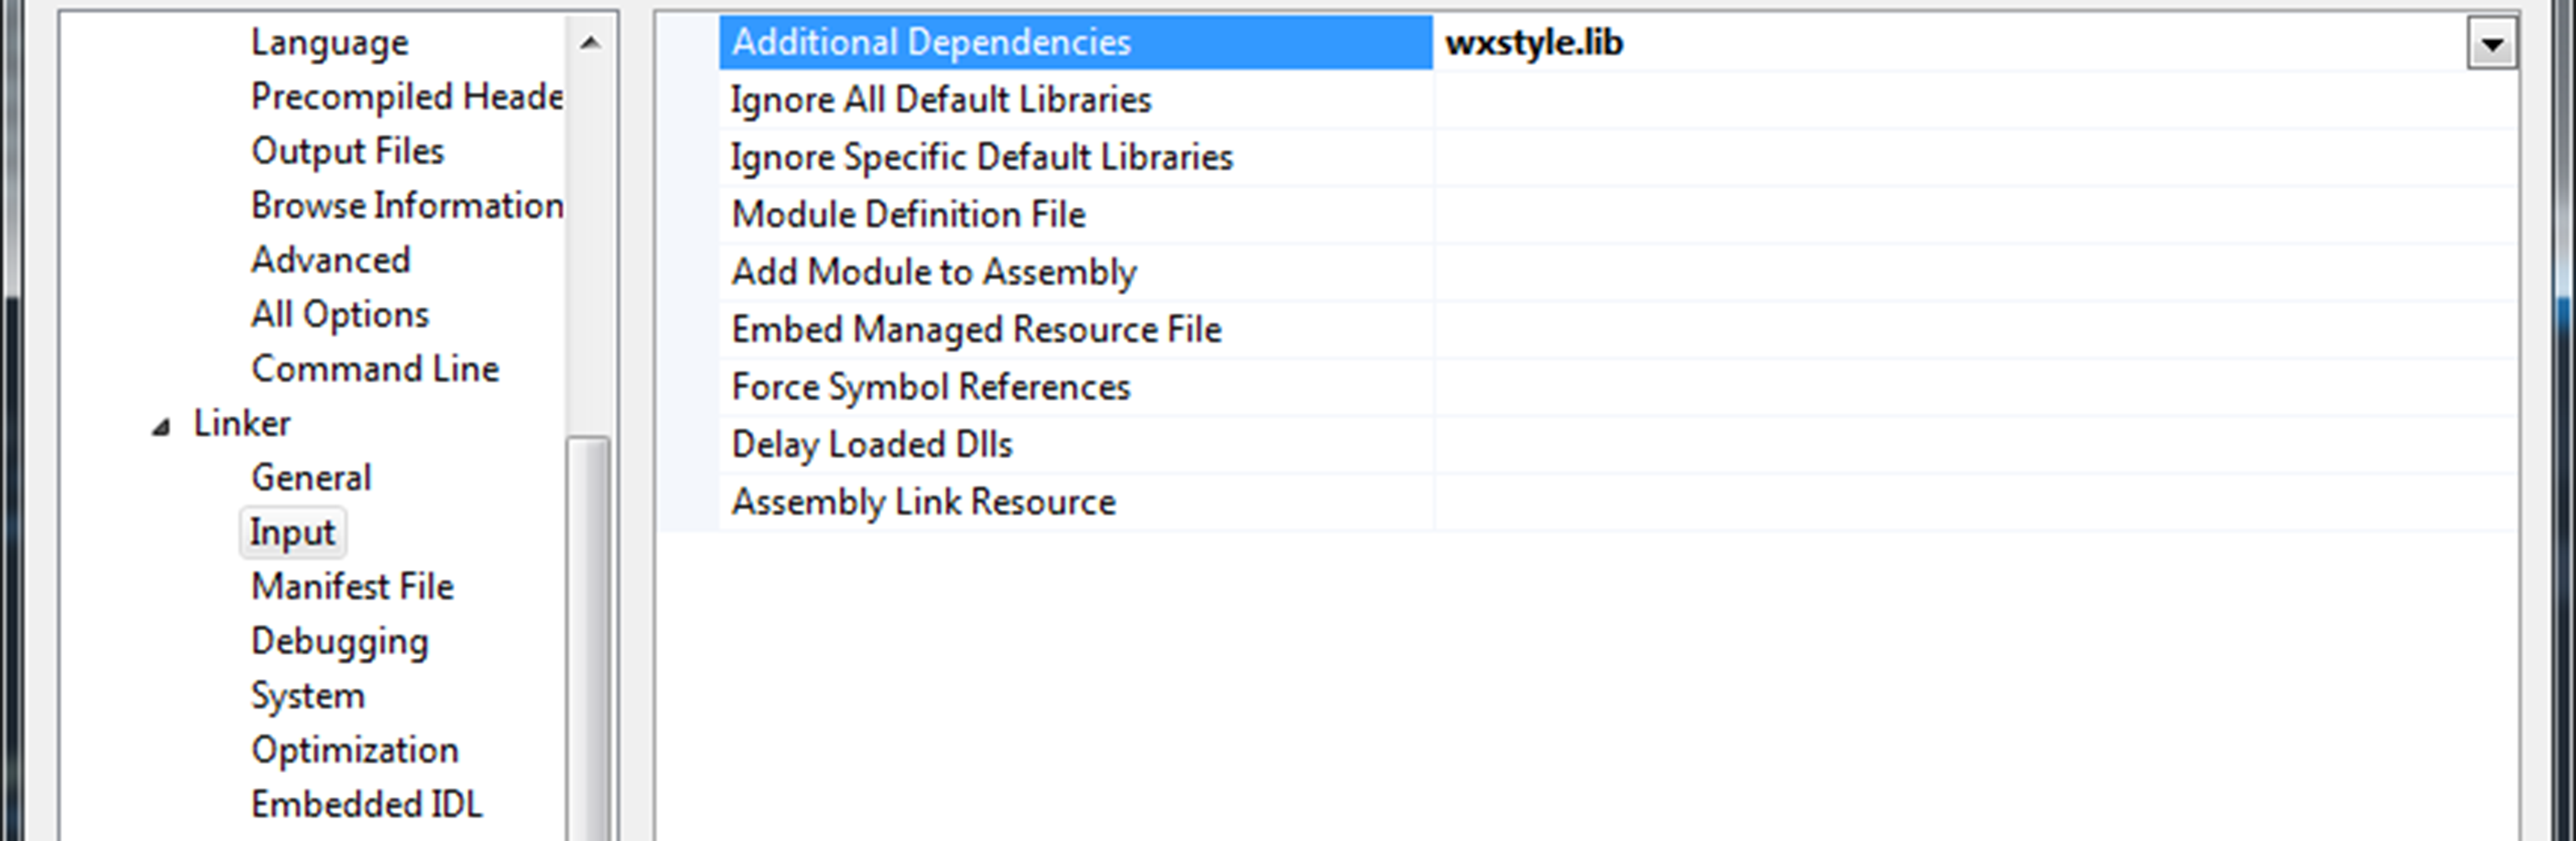
\includegraphics[width=15cm]{img/ch7_ide_lib_file.png}
\caption{Men'tionarea dependin'tei de fi'sierul binar wxstyle.lib}
\label{ch7_ide_lib_file}
\end{figure}

'In cele ce urmeaz'a, vom presupune c'a editorul Visual Studio 2012 recunoa'ste directivele de \emph{\#include} ce implic'a headere ale bibliotecii wxStyle, 'si g'ase'ste simbolurile compilate in fi'sierul binar wxstyle.lib

\subsection{Exemple de utilizare}

Scopul acestei sec'tiuni este de a prezenta sumar punctele de interes utiliz{\ia}nd exemple 'si explica'tii pentru cele mai des 'int{\ia}lnite situa'tii. Pentru informa'tii suplimentare, consulta'ti anexele A 'si B care prezint'a intreaga interfa't'a a bibliotecii si schema de descriere a limbajului utilizat la fi'sierele de stil. Mai ave'ti la dispozi'tie proiectul de prezentare numit \emph{demo} distribuit 'impreun'a cu aplica'tia.

\medskip

Din biblioteca \emph{wxStyle} pot fi folosite orice obiecte de interfa't'a oriunde 'in interiorul unei aplica'tii wxWidgets. Totu'si, este mai avantajoas'a folosirea unei ferestre stilizabile \emph{StyledFrame}. 'In interiorul acestei ferestre pot fi plasate at{\ia}t obiecte de interfa't'a wxWidgets c{\ia}t 'si componente stilizabile implementate in cadrul bibliotecii wxStyle. 'In plus fa't'a de ferestrele native implementate 'in wxWidgets, ferestrele stilizabile pot fi modificate 'in orice mod, de la schimbarea componentelor ce alc'atuiesc titlul ferestrei p{\ia}n'a la schimbarea fundalului cu o imagine transparent'a. Un exemplu ce construie'ste o fereastr'a \emph{StyledFrame} este prezentat 'in figura \ref{ex01}.

\begin{figure}[H]
\begin{lstlisting}[language=C++]
#include "StyledFrame.h"
using namespace wxstyle;
StyledFrame* CreateStyledFrame() {
	StyledFrame frame = new StyledFrame("Demo Board");
	frame->SetMinSize(wxSize(200, 200));
	frame->Show(true);
	return frame;
}
\end{lstlisting}
\caption{Exemplu de construire a unei ferestre \emph{StyledFrame}}
\label{ex01}
\end{figure}

Obiectele de interfa't'a se construiesc in mod similar celor implementate in wxWidgets, cu excep'tia faptului c'a acestea nu necesit'a asocierea unui identificator unic. Toate obiectele de interfa't'a au 'in comun un constructor ce specific'a obiectul p'arinte 'si textul obiectului (parametru op'tional). 'In cele mai multe situa'tii, p'arintele unui obiect va fi panoul de con'tinut al ferestrei care 'il con'tine. Exemplul din figura \ref{ex02} demonstreaz'a procesul de construire al unor obiecte de interfa't'a. Pozi'tionarea obiectelor 'in interiorul ferestrei se face folosind un obiect \emph{wxSizer} ata'sat panoului de con'tinut al ferestrei, a'sa cum se procedeaz'a 'in cadrul libr'ariei wxWidgets.

\begin{figure}[H]
\begin{lstlisting}[language=C++]
#include "StyledFrame.h"
#include "StyledLabel.h"
#Include "StyledButton.h"
using namespace wxstyle;
void CreateUIObjects(StyledFrame *frame) {
	wxPanel *contentPanel = frame->GetContentPanel();
	StyledLabel *label = new StyledLabel(contentPanel, "some text");
	StyledButton *button = new StyledButton(contentPanel, "some action");
}
\end{lstlisting}
\caption{Exemplu de construire al unor obiecte de interfa't'a}
\label{ex02}
\end{figure}

Stilizarea obiectelor de interfa't'a se face utiliz{\ia}nd structuri de tipul \emph{Style}. Acestea con'tin informa'tii necesare prezent'arii obiectelor 'in st'arile principale ale acestora: \emph{default}, \emph{disabled}, \emph{focused}, \emph{hovered}, \emph{pressed}. Un exemplu ce construie'ste un obiect de stil este prezentat in figura \ref{ex03}

\begin{figure}[H]
\begin{lstlisting}[language=C++]
#include "style/Style.h"
using namespace wxstyle;
Style* CreateStyle() {
	Style *result = new Style();
	DefinitionBundle bundle;
	bundle.SetFont(FontDefinition().SetFace("Tahoma").SetSize(3));
	bundle.SetForeground("#A2A2A2");
	bundle.SetOpaque(true);
	result.AddBundle(Style::CAT_DEFAULT, bundle);
	return result;
}
\end{lstlisting}
\caption{Exemplu de construire a unui stil}
\label{ex03}
\end{figure}

Defini'tiile necesare prezent'arii unui obiect sunt definite prin structuri precum \emph{FontDefinition}, \emph{ShadowDefinition} sau valori simple precum \emph{wxColour}. Acestea sunt agregate de structuri \emph{DefinitionBundle}. O astfel de structur'a este ata'sat'a unui stil la o categorie ce reprezint'a una din starile fundamentale ale unui obiect de interfa't'a.

\medskip

Deoarece construirea stilurilor prin cod este complicat'a, anevoioas'a 'si rigid'a, stilurile pot fi specificate prin fi'siere de stil numite \emph{stylesheets}. Acestea respect'a o structur'a clar'a, descris'a de schema XST prezent'a 'in Anexa A. Un exemplu de astfel de fi'sier este prezent 'in figura \ref{ex04}

\begin{figure}[H]
\begin{lstlisting}[language=XML]
<stylesheet name="test">
  <styles>
    <style name="default">
	  <default>
	    <font face="Tahoma" size="3"/>
		<insets rect="10, 3, 5, 3"/>
		<foreground color="#A2A2A2"/>
		<opacity value="true"/>
	  </default>
	</style>
  </styles>
</stylesheet>
\end{lstlisting}
\caption{Exemplu de fi'sier \emph{stylesheet}}
\label{ex04}
\end{figure}

Pentru a aduce 'in memorie stilurile con'tinute 'intr-un fi'sier de stiluri, se poate utiliza clasa \emph{XMLStylesheetLoader}. Rezultatul pars'arii unui astfel de fi'sier este o structur'a numit'a \emph{Stylesheet} ce con'tine o map'a de la numele unui stil la structura de stil. Un exemplu de astfel de parsare se g'ase'ste in figura \ref{ex05}

\begin{figure}[H]
\begin{lstlisting}[language=C++]
#include <string>
#include "style/XMLStylesheetLoader.h"
using namespace wxstyle;
void LoadStylesheet(const std::string& file) {
	XMLStylesheetLoader loader;
	Stylesheet stylesheet = loader.Load(file);
	Style defaultStyle = stylesheet.GetStyle("default");
}
\end{lstlisting}
\caption{Exemplu de parsarea a unui fi'sier de stiluri folosind \emph{XMLStylesheetLoader}}
\label{ex05}
\end{figure}

Asignarea unui stil la un obiect de interfa't'a se face utiliz{\ia}nd metoda \emph{SetStyle}. De asemenea, metoda \emph{GetStyle} este utilizat'a pentru ob'tinerea stilului asociat. Pentru extragerea structurii de tip \emph{StyleBundle} asociate unui obiect 'si care este corespunz'atoare st'arii acestuia se folose'ste metoda \emph{GetDefinitionBundle}. Aceast'a methoda combin'a bundle-ul default cu bundle-ul asociat st'arii pentru a genera un bundle gata de folosit. Un exemplu de utilizare al acestor metode se g'ase'ste in figura \ref{ex06}.

\begin{figure}[H]
\begin{lstlisting}[language=C++]
#include "style/Style.h"
#include "style/DefinitionBundle.h"
#include "StyledLabel.h"
using namespace wxstyle;
void SetStyleExample(const StyledLabel& label, const Style& style) {
	label.SetStyle(style);
	DefinitionBundle bundle = label.GetDefinitionBundle();
}
\end{lstlisting}
\caption{Exemplu de setarea a stilului unui obiect 'si extragerea unui \emph{DefinitionBundle}}
\label{ex06}
\end{figure}

Procesarea de evenimente se face diferit c{\ia}nd vine vorba de obiectele de interac'tiune ale bibliotecii wxStyle. Pentru ata'sarea unei metode de procesare unui eveniment utiliz'am obiecte de tipul listener asociate fiec'arei categorii de evenimente. Figura \ref{ex07} exemplific'a acest mecanism.

\begin{figure}[H]
\begin{lstlisting}[language=C++]
#include "StyledWindow.h"
using namespace wxstyle;
class ExampleMouseListener : public StyledWindow::MouseListener {
public:
	void MouseDown(const wxMouseEvent& mouseEvent) override {
		// Process the mouse event
	}
};
void RegisterEvent(const StyledWindow& window) {
	window->RegisterMouseListener(new ExampleMouseListener());
}
\end{lstlisting}
\caption{Exemplu de procesarea al evenimentelor generate de dispozitiv-ul mouse folosind obiecte de tip \emph{MouseListener}}
\label{ex07}
\end{figure}

Exemplele prezentate in aceast'a sec'tiune nu fac dec{\ia}t sa acopere suprafa'ta bibliotecii wxStyle. Posibilit'a'tile de stilizare 'si compunere a obiectelor de interfa't'a sunt nenum'arate. Pentru o documenta'tie complet'a, consulta'ti anexele A 'si B ce descriu 'in 'intregime formatul fi'sierelor de stiluri 'si a componentelor bibliotecii.
%
%% ==============================================================================
%%   Capitolul 8: Concluzii
%% ==============================================================================
%
\chapter{Concluzii}
\pagestyle{headings}

\section{Contribu'tia personal'a}

De'si no'tiunile de interfa't'a vizuala, tehnici de interac'tiune, prezentatori 'si metode de stilizare nu sunt deloc noi, proiectul de fa't'a adreseaz'a o problem'a practic'a 'si foarte specific'a: accea a lipsei de suport pentru obiecte de interfa't'a stilizabile incorporate 'intr-o bibliotec'a C++. 'In acest sens, contribu'tia mea a fost aceea de a utiliza tehnologii moderne (C++11, biblioteca boost, limbajul XML), no'tiuni abstracte (fi'siere de stil, liste de instruc'tiuni) 'si componente de infrastructur'a dovedite fiabile prin utilizarea lor 'in arhitecturi si biblioteci de succes (Unified Dimension) pentru a construi un set variat de obiecte de interfa't'a ce pot fi controlate deplin 'in ceea ce prive'ste prezentarea acestora.

\medskip

Ad'augarea suportului pentru stilizare, utiliz{\ia}nd fi'siere de stil, uneia dintre cele mai largi, portabile, open source 'si mature biblioteci de obiecte de interfa't'a pentru C++ este contribu'tia pe care acest proiect o aduce comunit'a'tii de dezvoltatori de aplica'tii vizuale.

\section{Analiza rezultatelor}

Biblioteca wxStyle a reu'sit s'a ating'a scopurile propuse 'in capitolul 2, mai exact:
\begin{enumerate}
\item Implementarea obiectelor de interfa't'a: \emph{fereastr'a}, \emph{label}, \emph{buton}, \emph{checkbox} 'si \emph{textbox}.
\item Stilizarea obiectelor de interfa't'a utiliz{\ia}nd proceduri de prezentare.
\item Stilizarea obiectelor de interfa't'a utiliz{\ia}nd fi'siere de stiluri.
\end{enumerate}

Din nefericire, exist'a unele probleme greu de rezolvat datorate bibliotecii wxWidgets, cum ar fi suportul incomplet 'si imprecis pentru calculul metricilor de text, lipsa de acurate'te a gradientelor, desenarea gre'sit'a a dreptunghiurilor rotunjite cu raza col'tului mic'a, etc. Aceste defecte pot fi corectate fie utiliz{\ia}nd o alt'a bibliotec'a pentru desenarea si analiza font-urilor, fie prin 'imbun'at'a'tirea bibliotecii wxWidgets.

Interfa't'a bibliotecii este inconsecvent'a pe alocuri, datorit'a deciziilor de design la nivel de implementare ce s-au schimbat pe parcursul proiectului. Acest lucru demonstreaz'a o lips'a de planificare ini'tial'a, care ar fi trebuit s'a descrie interfa't'a bibliotecii 'inaintea implement'arii acesteia.

\section{Dezvolt'ari ulterioare}

Distingem trei categorii de dezvolt'ari ulterioare pentru biblioteca wxStyle. Prima categorie presupune dezvoltarea bibliotecii 'intr-o direc'tie bine stabilit'a pentru a atinge un scop final. A doua categorie presupune dezvoltarea de tr'as'aturi 'si unelte auxiliare care ar putea face utilizarea libr'ariei mai u'soar'a, sau care pot m'ari avengura libr'ariei. O ultim'a categorie trateaz'a aplica'tii care ar beneficia 'in mod deosebit de contribu'tiile libr'ariei.

\subsection{Dezvoltarea planificat'a a bibliotecii}

Implementarea curent'a a bibliotecii wxStyle este doar un prim pas 'in direc'tia pe care a pornit. Scopul final al bibliotecii, care ar determina terminarea etapei de produc'tie a proiectului 'si intrarea 'in etapa de 'intre'tinere este portarea 'intregii libr'arii wxWidgets deasupra obiectelor de interfa't'a oferite de wxStyle. P{\ia}n'a a ajunge acolo 'ins'a, r'am{\ia}n foarte multe aspecte de acoperit. Dintre acestea, cele mai relevante sunt:

\begin{itemize}
\item Extinderea setului de obiecte de interfa't'a. Acest aspect presupune implementarea tuturor obiectelor de interfa't'a oferite de biblioteca wxWidgets \footnote{http://docs.wxwidgets.org/3.0/classwx\_window.html}. Acestea sunt 'in num'ar de aproximativ 30 'si includ: ferestre, meniuri, liste, arbori, obiecte de tip scrollbar, etc. De'si numeroase, obiectele de interfa't'a utilizate in mod frecvent sunt mai reduse. Implementarea stilizat'a a acestora este vital'a atingerii scopului final al bibliotecii wxStyle.
\item 'Imbun'at'a'tirea calit'a'tii 'si extinderea func'tionalit'a'tii obiectelor de interfa't'a curent implementate. Dintre aceste 'imbun'at'a'tiri, cele mai important'e sunt prezentate in figura \ref{fig0801}.
\item Fixarea problemelor introduse de biblioteca wxWidgets precum erorile de m'asurare a dimensiunilor textului. Aceast'a problem'a poate fi rezolvat'a prin utilizarea unei biblioteci specializate de desenare 'si procesare a textului precum \emph{FreeType} \footnote{http://freetype.org/}
\item Realizarea scopului original al bibliotecii printr-o implementare oficial'a a unei port'ari pentru biblioteca wxWidgets. A'sa cum se poate vedea 'in figura \ref{ch2_arhitectura_bloc}, blocul cel mai 'inalt corespunde unei extinderi a bibliotecii wxWidgets. Acest lucru ar face posibil'a utilizarea de componente stilizabile de c'atre aplica'tii care nu au fost original concepute s'a func'tioneze utiliz{\ia}nd biblioteca wxStyle.
\end{itemize}

\begin{center}
\begin{figure}[H]
    \centering
    \begin{tabular}{ |p{14cm}| }
        \hline
        \textbf{StyledFrame} \\
        Suport pentru redimensionare 'in toate cele 8 direc'tii \\
        Ad'augare de suport pentru icoan'a la nivelul titlului \\
        \hline
		\textbf{StyledTextBox} \\
        Suport pentru opera'tii de tip \emph{undo} 'si \emph{redo} \\
        Suport pentru mesaje ascunse (exemplu: c'asu'te text pentru parole) \\
		Suport pentru filtrarea de caractere acceptate (exemplu: casu'te numerice) \\
        \hline
    \end{tabular}
    \caption{Tr'as'aturi esen'tiale pentru dezvoltarea ulterioar'a a obiectelor de interfa't'a}
    \label{fig0801}
\end{figure}
\end{center}

\subsection{Dezvoltarea de unelte 'si tr'as'aturi auxiliare}

Alte tr'as'aturi de interes pentru biblioteca wxStyle care nu conduc dezvoltarea bibliotecii spre scopul original, dar ar 'imbun'at'a'ti semnificativ biblioteca sunt urm'atoarele:

\begin{itemize}
\item Ad'augarea de defini'tii pentru icoane construite prin font-uri iconografice. Font-uri precum \emph{Font Awesome}\footnote{http://fortawesome.github.io/Font-Awesome/}, \emph{Entypo}\footnote{http://www.entypo.com/} 'si altele ofer'a o gam'a foarte larg'a 'si variat'a de icoane. Ele sunt utilizate cu mult succes 'si popularitate 'in cadrul paginilor web. Introducerea lor 'in cadrul bibliotecii wxStyle ar 'insemna integrarea bibliotecii \emph{FreeType} pentru desenarea de caractere utiliz{\ia}nd font-uri 'inc'arcate in memorie. Avantajul acestui mecanism este posibilitatea gener'arii de icoane de orice dimensiuni, culori, asupra c'arora putem aplica orice efecte de rasterizare.
\item Extinderea fi'sierelor de stiluri cu suport pentru propriet'a'ti globale. Aceast'a tr'as'atura este deja par'tial implementat'a la nivel de cod dar nu a ajuns 'in specifica'tia fi'sierelor de stil. Ea const'a 'in posibilitatea definirii unei mape de propriet'a'ti globale pentru intregul fi'sier de stil. 'In prezen'ta acestei liste, defini'tiile de stil pot folosi ca valori pentru atribute nume de propriet'a'ti din mapa global'a. Se poate extrage astfel o tem'a universal'a la nivel de stylesheet. Acest lucru este posibil 'in momentul de fa't'a folosind no'tinuea de stiluri p'arinte.
\item Posibilitatea stiliz'arii p'ar'tilor componente ale unui obiect de interfa't'a. Obiectele de interfa't'a sunt 'in general compuse din mai multe p'ar'ti. De exemplu, un \emph{checkbox} este alc'atuit din c'asu'ta de bifat 'si textul descriptiv. Un alt exemplu mai concret este o list'a de elemente ce este format'a din: elementele listei, cutia 'in care sunt 'incadrate elementele 'si bara de navigare (scrollbar). Ar fi de preferat ca aceste componente s'a fie stilizate diferit. Deocamdat'a nu exist'a o descriere concret'a a cerin'tei pentru aceast'a tr'as'atur'a, deoarece este necesar'a o analiz'a mai detaliat'a a problemei, dar tr'as'atura 'in sine este foarte atr'ag'atoare pentru scopul bibliotecii.
\item Testarea automat'a a func'tionalit'a'tii obiectelor de interfa't'a. 'In urma analizei efectuate 'in capitolul 6, testarea la nivel de bibliotec'a se realizeaz'a 'in momentul de fa't'a 'in mod manual utiliz{\ia}nd aplica'tia demonstrativ'a. De'si exista avantaje la testarea manual'a, este de preferat o suit'a de teste automate care s'a garanteze corectitudinea func'tional'a a tuturor obiectelor de interfa't'a. Aceast'a suit'a de teste poate fi rulat'a periodic pentru a asigura consisten'ta calit'a'tii. Testarea automat'a la nivel de bibliotec'a poate fi realizat'a doar cu ajutorul unui framework de testare specific bibliotecii wxWidgets 'si a componentelor wxStyle. Un astfel de framework nu exist'a 'in momentul de fa't'a, dar biblioteca wxWidgets ofer'a un simulator de evenimente numit \emph{wxUIActionSimulator}. 'Incep{\ia}nd cu acest simulator, se poate construi un framework de testare specializat pentru obiectele de interfa't'a implementate 'in wxStyle.
\end{itemize}

\subsection{Aplica'tii cu senzor de contrast}
De'si orice aplica'tie poate beneficia 'in mod gratuit (f'ar'a efort) de tr'as'aturile libr'ariei wxStyle, unele nu ar putea fi construite utiliz{\ia}nd doar biblioteca wxWidgets. Consider c'a printre aceste aplica'tii se num'ar'a 'si aplica'tiile care ar utiliza patentul de'tinut de Apple numit \emph{"User interface contrast filter"} \cite{uicontrast}. 

\medskip

Astfel de aplica'tii pot reac'tiona la un senzor de lumin'a pentru a-'si schimba dinamic contrastul. Schibarea contrast-ului la nivel de aplica'tie necesit'a control granular asupra obiectelor de interfa't'a, lucru imposibil de realizat utiliz{\ia}nd doar biblioteca wxWidgets. Utiliz{\ia}nd 'in schimb biblioteca wxStyle, se pot scrie componente de prezentare specializate care s'a adjusteze culorile stilului 'inainte de a prezenta un obiect de interfa't'a. Pentru procesul efectiv de prezentare se poate folosi prezentatorul implicit, scopul prezentatorului specializat fiind doar adjustarea defini'tiilor incluse 'in stilul obiectului de interfa't'a.
%
%% ==============================================================================
%%   Bibliografie
%% ==============================================================================
%
\printbibliography[heading=bibintoc,title={Bibliografie}]
%
%% ==============================================================================
%%   Anexa A: Stylesheet XSD
%% ==============================================================================
%
\appendix
\chapter{Stylesheet XSD}
\pagestyle{headings}

\lstset{frame=none}

\begin{lstlisting}[language=XML]

<?xml version="1.0" encoding="UTF-8" standalone="no"?>
<xs:schema xmlns:xs="http://www.w3.org/2001/XMLSchema">

  <!-- Color Type -->
    <xs:simpleType name="t:color">
        <xs:restriction base="xs:string">
            <xs:pattern value="#[0-9A-Fa-f]{6}"/>
        </xs:restriction>
    </xs:simpleType>

  <!-- Font Weight Type -->
    <xs:simpleType name="t:fontWeight">
      <xs:restriction base="xs:string">
        <xs:enumeration value="normal"/>
        <xs:enumeration value="bold"/>
        <xs:enumeration value="light"/>
      </xs:restriction>
    </xs:simpleType>

  <!-- Font Style Type -->
    <xs:simpleType name="t:fontStyle">
      <xs:restriction base="xs:string">
        <xs:enumeration value="normal"/>
        <xs:enumeration value="italic"/>
      </xs:restriction>
    </xs:simpleType>

  <!-- Insets Type -->
    <xs:simpleType name="t:insets">
      <xs:list itemType="xs:integer">
        <xs:length value="4"/>
      </xs:list>
    </xs:simpleType>

    <!-- 2D Point Type -->
    <xs:simpleType name="t:point">
      <xs:list itemType="xs:integer">
        <xs:length value="2"/>
      </xs:list>
    </xs:simpleType>

  <!-- Unified Dimension Type -->
    <xs:simpleType name="t:unifiedDimension">
      <xs:documentation>
      The rules for pattern-matching a unified dimension are fairly 
      complex, and are ommited here. A unified dimension point matches 
      a string containing a relative and absolute componente separated 
      by a '%' character. Either the absolute or the relative component 
      might be ommited, but not both. Examples:

      1. 50%+3 - relative component of 0.5 and a absolute component of 3
      2. -200% - relative component of -2 and no absolute component
      3. +43 - absolute component of 43 and no relative component
      </xs:documentation>
      <xs:restriction base="xs:string"/>
    </xs:simpleType>

  <!-- Unified Dimension Point Type -->
    <xs:simpleType name="t:unifiedPoint">
      <xs:list itemType="unifiedDimension">
        <xs:length value="2"/>
      </xs:list>
    </xs:simpleType>

  <!-- Unified Dimension Rectangle Type -->
    <xs:simpleType name="t:unifiedRectangle">
      <xs:list itemType="unifiedDimension">
        <xs:length value="4"/>
      </xs:list>
    </xs:simpleType>

  <!-- Horizontal Anchor Type -->
  <xs:simpleType name="t:hAnchor">
      <xs:restriction base="xs:string">
      <xs:enumeration value="left"/>
      <xs:enumeration value="center"/>
      <xs:enumeration value="right"/>
      </xs:restriction>
  </xs:simpleType>

  <!-- Vertical Anchor Type -->
  <xs:simpleType name="t:vAnchor">
      <xs:restriction base="xs:string">
      <xs:enumeration value="top"/>
      <xs:enumeration value="center"/>
      <xs:enumeration value="bottom"/>
      </xs:restriction>
  </xs:simpleType>

  <!-- Boolean Type -->
  <xs:simpleType name="t:bool">
      <xs:restriction base="xs:string">
      <xs:enumeration value="true"/>
      <xs:enumeration value="false"/>
      </xs:restriction>
  </xs:simpleType>  

  <!-- Pen Style Type -->
  <xs:simpleType name="t:penStyle">
      <xs:restriction base="xs:string">
      <xs:enumeration value="solid"/>
      <xs:enumeration value="dot"/>
      </xs:restriction>
  </xs:simpleType>

  <!-- Font Definition -->
  <xs:complexType name="e:font">
    <xs:attribute name="face" type="xs:string" use="optional"/>
    <xs:attribute name="size" type="xs:integer" use="optional"/>
    <xs:attribute name="weight" type="t:fontWeight" use="optional"/>
    <xs:attribute name="style" type="t:fontStyle" use="optional"/>
  </xs:complexType>

  <!-- Shadow Definition -->
  <xs:complexType name="e:shadow">
    <xs:attribute name="offset" type="t:point" use="optional"/>
    <xs:attribute name="color" type="t:color" use="optional"/>
  </xs:complexType>

  <!-- Insets Definition -->
  <xs:complexType name="e:insets">
    <xs:attribute name="rect" type="t:insets" use="optional"/>
  </xs:complexType>

  <!-- Background Color Definition -->
  <xs:complexType name="e:background">
    <xs:attribute name="color" type="t:color" use="optional"/>
  </xs:complexType>

  <!-- Foreground Color Definition -->
  <xs:complexType name="e:foreground">
    <xs:attribute name="color" type="t:color" use="optional"/>
  </xs:complexType>

  <!-- Foreground Color Definition -->
  <xs:complexType name="e:opacity">
    <xs:attribute name="value" type="t:bool" use="optional"/>
  </xs:complexType>

  <!-- Icon Definition -->
  <xs:complexType name="e:icon">
    <xs:attribute name="name" type="xs:string" use="optional"/>
  </xs:complexType>

  <!-- Alignment Definition -->
  <xs:complexType name="e:alignment">
    <xs:attribute name="horizontal" type="t:hAnchor" use="optional"/>
    <xs:attribute name="vertical" type="t:vAnchor" use="optional"/>
  </xs:complexType>

  <!-- Draw Text Instruction -->
  <xs:complexType name="e:drawText">
    <xs:attribute name="message" type="xs:string" use="optional"/>
    <xs:attribute name="shadow-offset" type="t:point" use="optional"/>
    <xs:attribute name="shadow-color" type="t:color" use="optional"/>
    <xs:attribute name="font-face" type="xs:string" use="optional"/>
    <xs:attribute name="font-size" type="xs:integer" use="optional"/>
    <xs:attribute name="font-weight" type="t:fontWeight" use="optional"/>
    <xs:attribute name="font-style" type="t:fotnStyle" use="optional"/>
    <xs:attribute name="color" type="t:color" use="optional"/>
    <xs:attribute name="h-anchor" type="t:hAnchor" use="optional"/>
    <xs:attribute name="v-anchor" type="t:vAnchor" use="optional"/>
    <xs:attribute name="position" type="t:unifiedPoint" use="optional"/>
  </xs:complexType>

  <!-- Draw Shape Instruction -->
  <xs:complexType name="e:drawShape">
    <xs:attribute name="rect" type="t:unifiedRectangle" use="optional"/>
    <xs:attribute name="insets" type="t:insets" use="optional"/>
    <xs:attribute name="color" type="t:color" use="optional"/>
    <xs:attribute name="pen-size" type="xs:intege" use="optional"/>
    <xs:attribute name="pen-color" type="t:color" use="optional"/>
    <xs:attribute name="pen-style" type="t:penStyle" use="optional"/>
    <xs:attribute name="h-anchor" type="t:hAnchor" use="optional"/>
    <xs:attribute name="v-anchor" type="t:vAnchor" use="optional"/>
  </xs:complexType>

  <!-- Draw Image Instruction -->
  <xs:complexType name="e:drawImage">
    <xs:attribute name="image-path" type="xs:string" use="optional"/>
    <xs:attribute name="position" type="t:unifiedPoint" use="optional"/>
    <xs:attribute name="h-anchor" type="t:hAnchor" use="optional"/>
    <xs:attribute name="v-anchor" type="t:vAnchor" use="optional"/>
    <xs:attribute name="size" type="t:unifiedPoint" use="optional"/>
  </xs:complexType>

  <!-- Paint Definition -->
  <xs:complexType name="e:paint">
    <xs:sequence>
      <xs:element name="rect" type="e:drawShape">
      <xs:element name="ellipse" type="e:drawShape"/>
      <xs:element name="text" type="e:drawText"/>
      <xs:element name="image" type="e:drawImage"/>
    </xs:sequence>
  </xs:complexType>

  <!-- Definition Bundle -->
  <xs:complexType name="e:definitionBundle">
    <xs:sequence>
      <xs:element name="font" type="e:font"/>
      <xs:element name="shadow" type="e:shadow"/>
      <xs:element name="opacity" type="e:opacity"/>
      <xs:element name="insets" type="e:insets"/>
      <xs:element name="background" type="e:background"/>
      <xs:element name="foreground" type="e:foreground"/>
      <xs:element name="icon" type="e:icon"/>
      <xs:element name="alignment" type="e:alignment"/>
      <xs:element name="paint" type="e:paint"/>
    </xs:sequence>
  </xs:complexType>

  <!-- Style -->
  <xs:complexType name="e:style">
    <xs:attribute name="name" type="xs:string" use="optional"/>
    <xs:attribute name="parent" type="xs:string" use="optional"/>
    <xs:sequence>
      <xs:element name="default" type="e:definitionBundle"/>
      <xs:element name="pressed" type="e:definitionBundle"/>
      <xs:element name="hovered" type="e:definitionBundle"/>
      <xs:element name="focused" type="e:definitionBundle"/>
      <xs:element name="disabled" type="e:definitionBundle"/>
    </xs:sequence>
  </xs:complexType>

  <!-- Style List -->
  <xs:complexType name="e:styleList">
    <xs:sequence>
      <xs:element name="style" type="e:style"/>
    </xs:sequence>
  </xs:complexType>

  <!-- Map Entry -->
  <xs:complexType name="e:mapEntry">
    <xs:attribute name="class" type="xs:string" use="required"/>
    <xs:attribute name="style" type="xs:string" use="required"/>
  </xs:complexType>

  <!-- Object to Style Map -->
  <xs:complexType name="e:map">
    <xs:sequence>
      <xs:element name="item" tyle="e:mapEntry"/>
    </xs:sequence>
  </xs:complexType>

  <!-- Stylesheet -->
  <xs:element name="stylesheet">
    <xs:complexType>
      <xs:attribute name="name" type="xs:string" use="optional"/>
      <xs:sequence>
        <xs:element name="styles" type="e:styleList"/>
        <xs:element name="map" type="e:map" min_occurs="0" maxOccurs="1"/>
      </xs:sequence>
    </xs:complexType>
  </xs:element>

</xs:schema>
\end{lstlisting}

\end{document}
